
%% The first command in your LaTeX source must be the \documentclass command.
%\documentclass[sigconf,authorversion,nonacm]{acmart}%[sigconf,review]{acmart}

\documentclass[sigconf,nonacm]{acmart}%[sigconf,review]{acmart}
\usepackage{enumitem}
\usepackage{multirow}
\usepackage{verbatim}
%
%\ifdefined\directlua
%\edef\pdfcompresslevel{\pdfvariable compresslevel}
%\edef\pdfobjcompresslevel{\pdfvariable objcompresslevel}
%\fi
%\ifdefined\pdfcompresslevel
%\pdfcompresslevel=0
%\pdfobjcompresslevel=0
%\else
%\special{dvipdfmx:config z 0}
%\fi

%%%>
\usepackage[utf8]{inputenc}
% Information boxes
\newcommand*{\info}[4][16.3]{%
	\node [ annotation, #3, scale=0.65, text width = #1em,
	inner sep = 2mm ] at (#2) {%
		\list{$\bullet$}{\topsep=0pt\itemsep=0pt\parsep=0pt
			\parskip=0pt\labelwidth=8pt\leftmargin=8pt
			\itemindent=0pt\labelsep=2pt}%
		#4
		\endlist
	};
}
%%
%% \BibTeX command to typeset BibTeX logo in the docs
\AtBeginDocument{%
	\providecommand\BibTeX{{%
			\normalfont B\kern-0.5em{\scshape i\kern-0.25em b}\kern-0.8em\TeX}}}
%%
%% end of the preamble, start of the body of the document source.
%
%%Added by Dhaminda (not in template)
%\setcopyright{none}
%
\begin{document}
	
	%%
	\title{On Specifying for Trustworthiness}
	
	%%
	%% The "author" command and its associated commands are used to define
	%% the authors and their affiliations.
	%% Of note is the shared affiliation of the first two authors, and the
	%% "authornote" and "authornotemark" commands
	%% used to denote shared contribution to the research.
	\author{Dhaminda B. Abeywickrama}
	\affiliation{%
		\institution{Department of Computer Science, University of Bristol, UK}
		\streetaddress{Street address}
		\country{}}
	\email{dhaminda.abeywickrama@bristol.ac.uk}
	
	\author{Amel Bennaceur}
	\affiliation{%
		\institution{Department of Computing, Open University, UK}
		\streetaddress{Street address}
		\country{}}
	\email{amel.bennaceur@open.ac.uk}
	
	\author{Greg Chance}
	\affiliation{%
		\institution{Department of Computer Science, University of Bristol, UK}
		\streetaddress{Street address}
		\country{}}
	\email{greg.chance@bristol.ac.uk}
	
	\author{Yiannis Demiris}
	\affiliation{%
		\institution{Electrical and Electronic Engineering, Imperial College London, UK}
		\streetaddress{Street address}
		\country{}}
	\email{y.demiris@imperial.ac.uk}
	
	\author{Anastasia Kordoni}
	\affiliation{%
		\institution{Department of Psychology, Lancaster University, UK}
		\streetaddress{Street address}
		\country{}}
	\email{a.kordoni@lancaster.ac.uk}
	
	\author{Mark Levine}
	\affiliation{%
		\institution{Department of Psychology, Lancaster University, UK}
		\streetaddress{Street address}
		\country{}}
	\email{mark.levine@lancaster.ac.uk}
	
	\author{Luke Moffat}
	\affiliation{%
		\institution{Department of Sociology, Lancaster University, UK}
		\streetaddress{Street address}
		\country{}}
	\email{l.moffat1@lancaster.ac.uk}
	
	\author{Luc Moreau}
	\affiliation{%
		\institution{Department of Informatics, King's College London, UK}
		\streetaddress{Street address}
		\country{}}
	\email{luc.moreau@kcl.ac.uk}
	
	\author{Mohammad Reza Mousavi}
	\affiliation{%
		\institution{Department of Informatics, King's College London, UK}
		\streetaddress{Street address}
		\country{}}
	\email{mohammad.mousavi@kcl.ac.uk}
	
	\author{Bashar Nuseibeh}
	\affiliation{%
		\institution{Department of Computing, Open University, UK}
		\streetaddress{Street address}
		\country{}}
	\email{b.nuseibeh@open.ac.uk}
	
	\author{Subramanian Ramamoorthy}
	\affiliation{%
		\institution{School of Informatics, University of Edinburgh, UK}
		\streetaddress{Street address}
		\country{}}
	\email{s.ramamoorthy@ed.ac.uk}
	
	\author{Jan Oliver Ringert}
	\affiliation{%
		\institution{Dept. of Computer Science, Bauhaus University Weimar, Germany}
		\streetaddress{Geschwister-Scholl-Strasse 8}
		\country{}}
	\email{jan.ringert@uni-weimar.de}
	
	\author{James Wilson}
	\affiliation{%
		\institution{Department of Engineering Maths, University of Bristol, UK}
		\streetaddress{Street address}
		\country{}}
	\email{j.wilson@bristol.ac.uk}
	
	\author{Shane Windsor}
	\affiliation{%
		\institution{Department of Aerospace Engineering, University of Bristol, UK}
		\streetaddress{Street address}
		\country{}}
	\email{shane.windsor@bristol.ac.uk}
	
	\author{Kerstin Eder}
	\affiliation{%
		\institution{Department of Computer Science, University of Bristol, UK}
		\streetaddress{Street address}
		\country{}}
	\email{kerstin.eder@bristol.ac.uk}
	
	%%
	%% By default, the full list of authors will be used in the page
	%% headers. Often, this list is too long, and will overlap
	%% other information printed in the page headers. This command allows
	%% the author to define a more concise list
	%% of authors' names for this purpose.
	\renewcommand{\shortauthors}{D. B. Abeywickrama et al.}
	
	%%
	%% The abstract is a short summary of the work to be presented in the
	%% article.
	\begin{abstract}
As autonomous systems (AS) are becoming part of our daily lives, ensuring their trustworthiness is crucial. There are a number of techniques for demonstrating trustworthiness, and common to all these techniques is the need to formulate \emph{specifications}. The main contribution of this roadmap paper is to go beyond summarising the current state-of-the-art and discussing its limitations, by identifying key challenges for specifying for trustworthiness in AS. Instead of dealing with a wide range of topics, we focus on several key open research problems that are being investigated within the UKRI Trustworthy Autonomous Systems (TAS) programme in relation to governance and regulation, functionality, resilience, trust, security, and verifiability. 
As another key contribution, we discuss specification challenges that are unique to key AS domains currently being investigated within our community. 
This roadmap paper is a result of a workshop we conducted on specifying for trustworthiness in AS in September 2021.
% REVIEWED abstract:		
%		As autonomous systems are becoming part of our daily lives, ensuring their trustworthiness is crucial. 
%		There are a number of techniques for demonstrating trustworthiness. 
%		Common to all these techniques is the need to articulate \emph{specifications}. 
%		In this paper, we take a broad view of specification, concentrating on top-level requirements including but not limited to functionality, safety, security and other non-functional properties. 
%		The main contribution of this article is a set of high-level intellectual challenges for the autonomous systems community related to specifying for trustworthiness.
%		We also describe unique specification challenges concerning a number of application domains for autonomous systems.
	\end{abstract}
	
	%%
	%% The code below is generated by the tool at http://dl.acm.org/ccs.cfm.
	%% Please copy and paste the code instead of the example below.
	%%
	\begin{CCSXML}
		<ccs2012>
		<concept>
		<concept_id>10010147.10010178</concept_id>
		<concept_desc>Computing methodologies~Artificial intelligence</concept_desc>
		<concept_significance>500</concept_significance>
		</concept>
		<concept>
		<concept_id>10011007.10011074.10011075.10011076</concept_id>
		<concept_desc>Software and its engineering~Requirements analysis</concept_desc>
		<concept_significance>500</concept_significance>
		</concept>
		<concept>
		<concept_id>10011007.10010940</concept_id>
		<concept_desc>Software and its engineering~Software organization and properties</concept_desc>
		<concept_significance>500</concept_significance>
		</concept>
		<concept>
		<concept_id>10011007.10010940.10010992</concept_id>
		<concept_desc>Software and its engineering~Software functional properties</concept_desc>
		<concept_significance>500</concept_significance>
		</concept>
		<concept>
		<concept_id>10011007.10010940.10011003</concept_id>
		<concept_desc>Software and its engineering~Extra-functional properties</concept_desc>
		<concept_significance>500</concept_significance>
		</concept>
		</ccs2012>
	\end{CCSXML}
	
	\ccsdesc[500]{Computing methodologies~Artificial intelligence}
	\ccsdesc[500]{Software and its engineering~Requirements analysis}
	\ccsdesc[500]{Software and its engineering~Software organization and properties}
	\ccsdesc[500]{Software and its engineering~Software functional properties}
	\ccsdesc[500]{Software and its engineering~Extra-functional properties}
	
	%\ccsdesc[500]{Computing methodologies~Artificial intelligence}
	
	%%
	%% Keywords. The author(s) should pick words that accurately describe
	%% the work being presented. Separate the keywords with commas.
	\keywords{autonomous systems, trust, specification}
	
	%%
	%% This command processes the author and affiliation and title
	%% information and builds the first part of the formatted document.
	\maketitle
	
	\section{Introduction}\label{introduction}
	Autonomous systems (AS) are systems that involve software applications, machines and people, which are capable of taking actions with no or little human supervision~\cite{Murukannaiah2020}. 
	Soon, AS will no longer be confined to safety-controlled industrial settings. 
	Instead, they will increasingly become part of our daily lives having matured across different domains like driverless cars, healthcare robotics and uncrewed aerial vehicles. 
	
	\emph{Trust} may vary, as it can be gained and lost over time. Different research disciplines define trust in different ways. This article focuses on the notion of trust that concerns the relationship between humans and AS. 
	AS are considered \emph{trustworthy} when the design, engineering, and operation of these systems generate positive outcomes and mitigate outcomes which can be harmful~\cite{Naiseh2022}.
	Trustworthiness of AS can be dependent on many factors such as: (i) explainability, accountability and understandability to different users; (ii) robustness of AS in dynamic and uncertain environments; (iii) assurance of their design and operation through verification and validation (V\&V) activities; (iv) confidence in their ability to adapt their functionality as required; (v) security against attacks on the systems, users, and deployed environment; (vi) governance and regulation of their design and operation; and (vii) consideration of ethics and human values in their deployment and use~\cite{Naiseh2022}. 
		
	There are various techniques for demonstrating trustworthiness of AS, such as synthesis, formal verification at design time, runtime verification or monitoring, and test-based methods. 
	But, common to all these techniques is the need to formulate \emph{specifications}. 	
	According to the ISO standard for systems and software engineering vocabulary~\cite{ISO24765:2017}, a \emph{specification} is a detailed formulation that provides a definitive description of a system for the purpose of developing or validating the system. 
%
% REVIEWED version:	
%	Writing specifications that inspire trust is challenging~\cite{Kress-Gazit2021}. 
%	A human may trust an AS to perform its actions, if it demonstrably acts in an effective and safe manner. 
%	Thus, the AS not only needs to be safe and effective, but also needs to be perceived as such by humans. 
%	%
%	In the same manner, in human-robot interaction, it is equally important to ensure that the AS can trust humans. 
%	%	
%	To address this, specifications will need to go beyond typical functionality and safety aspects. Thus, in this context, we take a broad view of specification, concentrating on top-level requirements including but not limited to functionality, safety, security and other non-functional properties that contribute to trustworthiness of AS. 
%	Also, we intentionally leave the discussion on the formalisation of these specifications for the future, when understanding of what is required to specify for trustworthiness is more mature.
	Writing specifications that inspire trust is challenging~\cite{Kress-Gazit2021}. 
	A human may trust an AS to perform its actions, if it demonstrably acts in an effective and safe manner. 
	Thus, the AS not only needs to be safe and effective, but also needs to be perceived as such by humans. 
	%
	In the same manner, in human-robot interaction, it is equally important to ensure that the AS can trust humans. 
	%	
	To address this, specifications will need to go beyond typical functionality and safety aspects. 	

	% REVISION - Dhaminda 2022/11/25	
	In the UK Research and Innovation (UKRI) Trustworthy Autonomous Systems (TAS) programme, we conduct cross-disciplinary fundamental research to ensure that AS are safe, reliable, resilient, ethical, and trusted. 
	TAS is organised around six research projects called Nodes and a Hub, and each Node focuses on individual aspects of trust in AS, such as governance and regulation, functionality, resilience, trust, security, and verifiability. 

	% REVISION - Dhaminda 2022/11/25	
	%	Undertaking a community approach, this roadmap paper is a result of a workshop, which gathered a diverse group of high-quality researchers from all the TAS Nodes and the Hub in Sept. 2021. 
	Undertaking a community approach, this roadmap paper is a result of the specifying for trustworthiness workshop held during the TAS All Hands Meeting in Sept. 2021. 
	The workshop gathered a diverse group of high-quality researchers from all the six TAS Nodes and the Hub. 
	Co-authored by a representative sample of the AS community in the UK, the main contribution of this roadmap paper is to go beyond summarising the current state-of-the-art and discussing its limitations, by identifying key challenges for specifying for trustworthiness in AS. 
	We take a broad view of specification, concentrating on top-level requirements including but not limited to functionality, safety, security, and other non-functional properties that contribute to trustworthiness of AS. 
	Also, we intentionally leave the discussion on the formalisation of these specifications for the future, when understanding of what is required to specify for trustworthiness is more mature.	
	As another key contribution, we discuss specification challenges that are unique to a representative set of AS domains currently being investigated within our community. 
	%Instead of dealing with a wide range of topics associated with the field, this paper focuses on several key open research problems and challenges that are currently being investigated within the different Nodes of the UKRI Trustworthy Autonomous Systems (TAS) programme in relation to governance and regulation, functionality, resilience, trust, security, and verifiability. 
	%This roadmap paper is a result of a workshop we conducted on specifying for trustworthiness in AS which took place in September 2021.
	
	In order to motivate and present a set of research challenges associated with specifying for trustworthiness in AS, this paper is divided into two parts. Section~\ref{as-domains} discusses a number of AS domains, each with its unique specification challenges. Section~\ref{as-challenges} presents several key open research problems that are currently being investigated within our community. Finally, Section~\ref{conclusions} summarises our findings.
	%
	% REVIEWED version:	
	%	In this paper, we explore what it means to specify for trustworthiness, considering a number of AS domains, each with its unique specification challenges. We then present a set of intellectual challenges for the AS community comprising both academia and industry, specifically focusing on specification for trustworthy AS.
	%%-----------------------------------------------------------------------------------------------------------------------------------------------------------------------------------------------------------------------------
	
	\section{Autonomous Systems Domains and their Specification Challenges}\label{as-domains}
In this paper, by taking inspiration from \cite{Schneiders2022}, we classify the AS domains based on two criteria: the number of autonomous agents (single or multiple), and whether there are humans involved in the interaction. Accordingly, typical domains of AS can take one of four forms: (i) a single autonomous agent (e.g. automated driving, UAV); (ii) a group of autonomous agents (e.g. swarms); (iii) an autonomous agent with a human (e.g. AI in healthcare, human-robot interaction); and (iv) a group of autonomous agents with humans (e.g. emergency situations and disaster relief). First and foremost, this exercise is not intended to be exhaustive. We now discuss specification challenges of a representative set of domains which are being investigated within our community in TAS (see Table.~\ref{AS-challenges}). 
%	In this section, we discuss the specification challenges of a number of different AS domains (see Fig.~\ref{AS-challenges}).	
%	\begin{figure*}
%		\centering
%		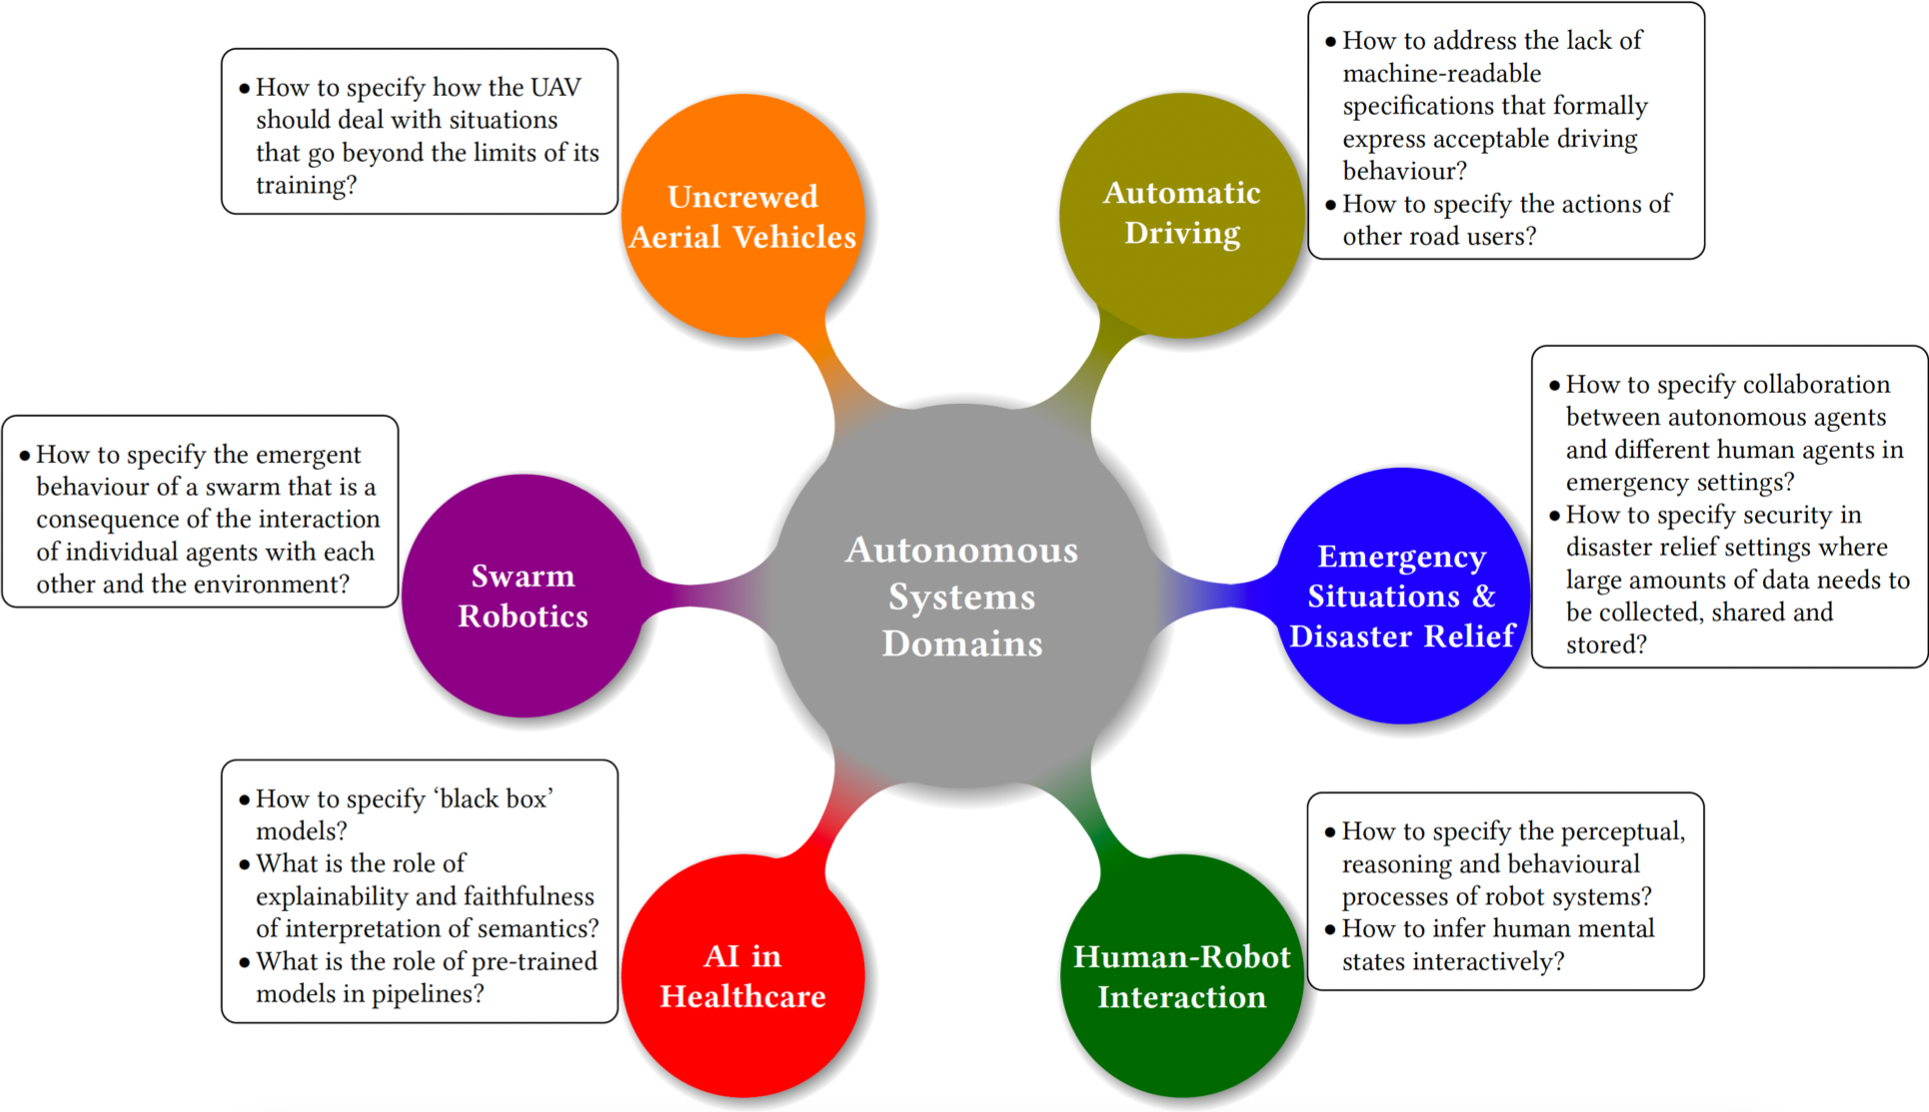
\includegraphics[width=0.9\textwidth]{figures/AS-Challenges.png}
%		\caption{AS domains and their specification challenges.}
%		\label{AS-challenges}
%	\end{figure*}
	
	\begin{itemize}[leftmargin=0.5cm]
		\item \textbf{Automated Driving} 
	\end{itemize}
	Automated driving (self-driving) refers to a class of AS that vary in the extent to which they make decisions independently (SAE J3016 standard taxonomy). The higher levels of autonomy, levels 3-5, refer to functionality ranging from traffic jam chauffeur to completely hands-free driving in all conditions. Despite an explosion of activity in this domain in recent years, the majority of systems being considered for deployments depend on careful delineation of the operation design domain (ODD) to make the specification of appropriate behaviour tractable. Even so, the specification problem remains difficult for a number of reasons. 
	%
	Firstly, traffic regulations are written in natural language, ready for human interpretation. Although the highway code rules are intended for legal enforcement, they are not specifications that are suitable for machines. 
	%
	There typically are many exceptions, context-dependent conflicting rules and guidance of an `open nature', all of these require interpretation in context. 
	Driving rules can often be vague or even conflicting and may need a base of knowledge to interpret the rule given a specific context. The UK Highway Code Rule 163 states that after you have started an overtaking manoeuvre you should ``move back to the left as soon as you can but do not cut in''~\cite{UKHighwayCode22}. A more explicit specification of driving conduct (e.g. Rule 163) to something more machine interpretable that captures the appropriate behaviour presents a challenge to this research area. When people are taught to perform this activity a significant portion of the time is spent in elaborating these special cases, and much of the testing in the licensing regime is aimed at probing for uniformity of interpretation. How best to translate these human processes into the AS domain is important not only for achieving safety but also acceptability.
	Secondly, driving in urban environments is an intrinsically interactive activity, involving several actors whose internal states may be opaque to the automated vehicle. As an example, the UK Highway Code asks drivers to not ``pull out into traffic so as to cause another driver to slow down''. 
	%
	Without further constraint on what the other drivers could possibly do, specifying appropriate behaviour becomes difficult, and any assumptions made in that process would call into question the safety of the overall system when those assumptions are violated. 
	Thus, two key challenges in the area of automated driving are the lack of machine-readable specifications that formally express acceptable driving behaviour and the need to specify the actions of other road users (see also Table.~\ref{AS-challenges}). To some extent, these issues arise in all open environments. However, in autonomous driving, the task is so intricately coupled with the other actors that even the default assumptions may not be entirely clear, and the relative variation in behaviour due to different modelling assumptions could be qualitatively significant.
	
	%Original contribution by the author/s:
	%Autonomous driving refers to a class of autonomous systems that vary in the extent to which they make decisions independently (SAE J3016 standard taxonomy). The higher levels of autonomy, levels 3-5, refer to functionality ranging from traffic jam chauffeur to completely hand-free driving in all conditions. Despite an explosion of activity in this domain in recent years, the majority of systems being considered for deployments depend on careful delineation of the operating design domain (ODD) to make the specification of appropriate behaviour tractable. Even so, the specification problem remains difficult for a number of reasons. Firstly, the traffic regulations which were originally written in plain English, assuming human interpretation rather than machine implementation. So, although the highway codes are written with a view to legal enforcement, they are not formal specifications. This means that the code contains many exceptions, rule conflicts and guidance of an `open texture', requiring interpretation in context. An example might be the specification of ``right of way''. Secondly, driving in urban environments is an intrinsically interactive and multi-agent activity, involving several actors whose internal states may be opaque to the autonomous vehicle. As an example, the UK highway code asks drivers to not ``pull out into traffic so as to cause another driver to slow down''. Without further constraint on what the other drivers could possibly do, specifying appropriate behaviour would be difficult, and any assumptions made in that process would call into question the safety of the overall system when those assumptions are violated. 

%\begin{table}
%	\caption{AS domains and their specification challenges.} \label{AS-challenges}   
%	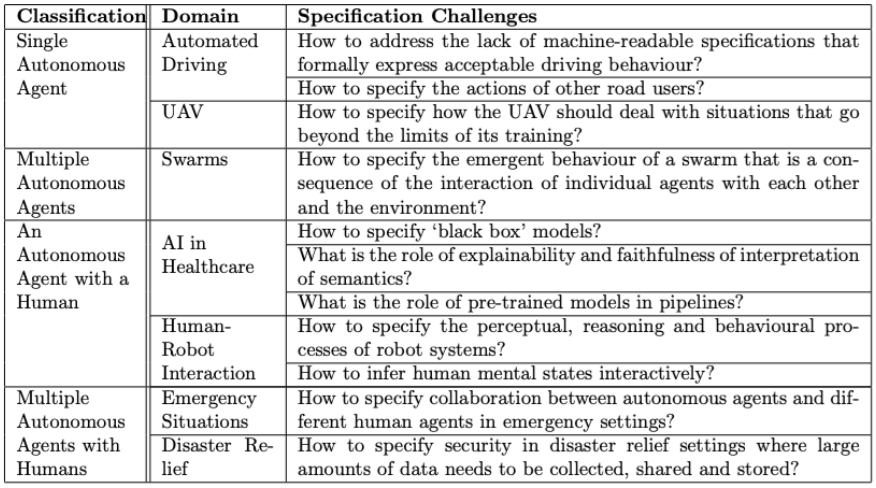
\includegraphics[width=0.5\textwidth]{figures/Domains.png}
%\end{table} 

%	\begin{figure}
%	\centering
%	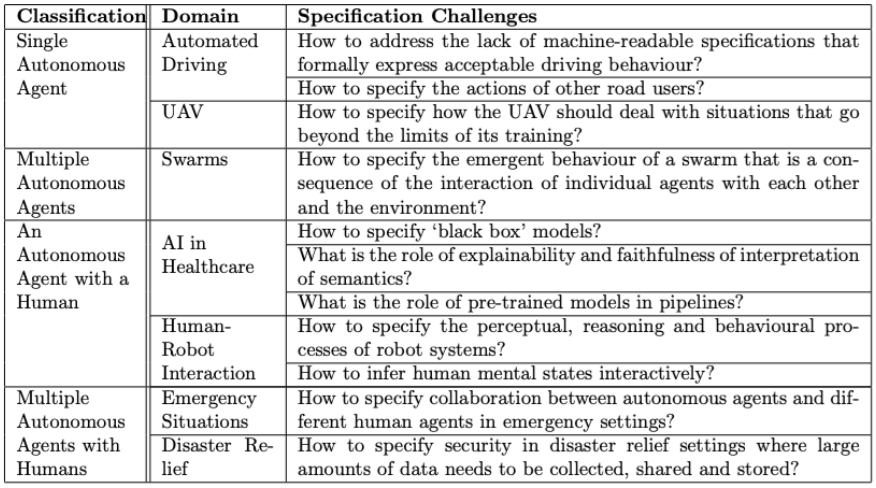
\includegraphics[width=0.5\textwidth]{figures/Domains.png}
%	\caption{AS domains and their specification challenges.}
%	\label{AS-challenges}
%\end{figure}		
	%%------------------------------------------------------------------------------------------------------------------------------------------------------------------------------------------------------------------------------
\begin{itemize}[leftmargin=0.5cm]
	\item \textbf{Uncrewed Aerial Vehicles}
\end{itemize}
An uncrewed aerial vehicle (UAV) or drone is a type of aerial vehicle that is capable of autonomous flight without a pilot on board. UAVs are increasingly being applied in diverse applications, such as logistics services, agriculture, emergency response, and security. Specification of the operational environment of UAVs is often challenging due to the complexity and uncertainty of the environments that UAVs need to operate in. 
For instance, in parcel delivery using UAVs in urban environments, there can be uncertain flight conditions (e.g.\ wind gradients), and highly dynamic and uncertain airspace (e.g.\ other UAVs in operation). 
Recent advances in machine learning offer the potential to increase the autonomy of UAVs in uncertain environments by allowing them to learn from experience. 
For example, machine learning can be used to enable UAVs to learn novel manoeuvres to achieve perched landings in uncertain windy conditions~\cite{Fletcher2021}. 
In these contexts, a key challenge is how to specify how the system should deal with situations that go beyond the limits of its training (Table.~\ref{AS-challenges}).

%Original contribution by the author/s:
%A uncrewed aerial vehicle (UAV) or drone is a type of aerial vehicle that is capable of autonomous flight without a pilot on board.
%As UAVs are increasingly being applied in diverse areas of applications, such as logistics services, agriculture, emergency response, and security, ensuring their trustworthiness is crucial \cite{Ukaegbu2021}.  
%Specification of operational environments of UAVs is challenging mainly for two reasons. 
%First, the unclear and uncertain government regulations may change over time. 
%Second, the complexity and uncertainty of the operational environment  itself is a challenge. 
%For instance, in parcel delivery using UAVs in urban environments, there can be uncertain flight conditions (e.g. wind gradients), and highly dynamic and uncertain airspace (e.g. other UAVs in operation). 
%
%The recent advances in machine learning offer the potential to increase the autonomy of UAVs by allowing them to learn from experience. 
%For example, machine learning can be used to stabilize the flight which can greatly improve performance in gusty urban wind conditions. 
%When one considers the conventional flight controller of a UAV, it can include several measures, such as risetime, overshoot, settling time, and steady-state error \cite{Kada2011}.
%The goals of these specification measures are to ensure that the control system is stable and robust; disturbance attenuation against environmental uncertainty; smooth and rapid responses to set-point changes; and steady-state accuracy. 
%In this context, a key challenge is how do we specify a UAV should deal with situations that go beyond the limits of its training?
%%------------------------------------------------------------------------------------------------------------------------------------------------------------------------------------------------------------------------------
% Shane comment: I don't think this fits the flow of the paper well at all as it is not an AS domain and it says nothing about specification - I think we should remove and have commented out.
%	\begin{itemize}[leftmargin=0.5cm]
	%		\item \textbf{Policy Development}
	%	\end{itemize}
%	Policy can be seen by research domains as slow moving and hard to penetrate. 
%	Beyond policy recommendations as research outcomes, what channels exist for informing policy development for AS? 
%	Through the \emph{isITethical} platform \cite{isITethical}, some work has been completed in collaboration with engineers, designers, programmers, policy advocates, publics and non-governmental organizations. 
%	One important aspect of this work is the use of creative and participatory methods to facilitate conversations and ways of thinking about ethics and security in the future of AS operations. 
%	These methods can help to recognise and sustain a need to get many voices into the same room to think not just how these technologies should be used when they arrive, but also how they should be designed in the first place. 
%	Instilling a sense of ethics through security that is maintained through the design process can generate good use cases that inform policy and standards that endure in future AS development. 
%	We must the think about whether AS are worthy of our trust, and also whether we are worthy of their use.

%-------------------------
%Revised version by author on December 14, 2021:
%Policy can be seen by research domains as slow moving, and hard to penetrate. Beyond policy recommendations as research outcomes, what channels exist for informing policy development around autonomous systems? Through the isITethical platform [1], some work has been completed in collaboration with engineers, designers, programmers, policy advocates and publics and non-governmental organizations. One legacy from this work that has transferred to TAS-S, is the use of creative and participatory methods to facilitate conversations and ways of thinking about ethics and security in the future of AS operations. These methods can help to recognise and sustain a need to get many voices in to the same room as possible, in order to think about not just how these devices or technologies should be used when they arrive, but how these devices should be designed in the first place. Instilling a sense of ethics through security, that is maintained through the design process, can generate good use cases that inform policy and standards the endure in future AS development. We must the think about whether AS are worthy of our trust, and also whether we are worthy of their use.
%-------------------------
%Original contribution by the author/s on October 27, 2021:
%Policy can be seen by research domains as slow moving, and hard to penetrate. Beyond policy recommendations as research outcomes, what channels exist for informing policy development around autonomous systems? Through the \emph{isITethical} platform \cite{isITethical}, some work has been completed in collaboration with engineers, designers, programmers, policy advocates and publics and non-governmental organizations. One legacy from this work that has transferred to TAS-S, is the use of creative and participatory methods to facilitate conversations and ways of thinking about ethics and security in the future of AS operations. These methods can help to recognise and sustain a need to get many voices in to the same room as possible, in order to think about not just how these devices or technologies should be used when they arrive, but how these devices should be designed in the first place. Instilling a sense of ethics through security, that is maintained through the design process, can generate good use cases that inform policy and standards the endure in future AS development. We must the think about whether AS are worthy of our trust, and also whether we are worthy of their use.
	
%%------------------------------------------------------------------------------------------------------------------------------------------------------------------------------------------------------------------------------
\begin{itemize}[leftmargin=0.5cm]
	\item \textbf{Swarm Robotics}
\end{itemize}
Swarm robotics provides an approach to the coordination of large numbers of robots, which is inspired from the observation of social insects \cite{Sahin2005}. Three desirable properties in any swarm robotics system are robustness, flexibility and scalability. 
The functionality of a swarm is emergent (e.g. aggregation, coherent ad hoc network, taxis, obstacle avoidance and object encapsulation \cite{Winfield2006}), and evolves based on the capabilities of the robots and the numbers of robots used. 
The overall behaviours of a swarm are not explicitly engineered in the system, but they are an emergent consequence of the interaction of individual agents with each other and the environment.
This emergent functionality poses a challenge for specification. The properties of individual robots can be specified in a conventional manner, yet it is the emergent behaviours of the swarm that determine the performance of the system as a whole. The challenge is to develop specification approaches that specify properties at the swarm level that can be used to develop, verify and monitor swarm robotic systems.

%Original contribution by the author/s:	
%Swarm robotics provides an approach to the coordination of large numbers of robots, which is inspired from the observation of social insects \cite{Sahin2005}. 
%Three desirable properties in any swarm robotics system are robustness, flexibility and scalability. 
%In \cite{Sahin2005}, a set of criteria is proposed for distinguishing swarm robotic research from multi-robot systems. 
%The individual robots that make up the swarm need to be autonomous. Also, there need to be a large number of robots; a few homogenous groups of robots; relatively incapable or inefficient robots; and robots with local sensing and communication capabilities. 
%
%The functionality of a swarm is emergent (e.g. aggregation, coherent ad hoc network, taxis, obstacle avoidance and object encapsulation \cite{Winfield2006}), and evolves based on the capabilities of the robots and the numbers of robots used. 
%The overall desired behaviours of a swarm are not explicitly engineered in the system, but they are an emergent consequence of the interaction of individual agents with each other and the environment.
%This evolving functionality across many individual robots poses a challenge in how to specify a swarm that is safe, trustworthy by design, useful, and acceptable to users?
%%------------------------------------------------------------------------------------------------------------------------------------------------------------------------------------------------------------------------------
\begin{itemize}[leftmargin=0.5cm]
	\item \textbf{Human-Robot Interaction}%{Trustworthy Interactive Robot Systems}
\end{itemize}
Interactive robot systems aim to complete their tasks while explicitly considering states, goals and intentions of the human agents they collaborate with, and aiming to calibrate the trust humans have for them to an appropriate level. This form of human-in-the-loop real-time interaction is required in several application domains including assistive robotics for activities of daily living \cite{GaoEtAl2020}, healthcare robotics, shared control of smart mobility devices \cite{SohDemiris2015}, and collaborative manufacturing among others. Most specification challenges arise from the need to provide specifications for the perceptual, reasoning and behavioural processes of robot systems that will need to acquire models of, and deal with, the high variability exhibited in human behaviour. 
% Yiannis Demiris's edited last sentence in response to reviewer comments:
While several human-in-the-loop systems employ mental state inference, the necessity for interactively performing such inference (including as beliefs and intentions), typically through sparse and/or sensor data from multimodal interfaces, imposes further challenges for the principled specification of human factors and data-driven adaptation processes in robots operating in close proximity to humans, where safety and reliability are of particular importance. 
%The necessity to infer human mental states (such as beliefs and intentions) interactively, typically through sparse and/or sensor data from multimodal interfaces, imposes further challenges for the principled specification of human factors and data-driven adaptation processes in robots operating in close proximity to humans, where safety and reliability are of particular importance. 

%Original contribution by the author/s:
%Trustworthy Interactive Robot Systems aim to complete their tasks while explicitly considering states, goals and intentions of the human agents they collaborate with, and aiming to calibrate the trust humans have for them to an appropriate level.  This form of human-in-the-loop real-time interaction is required in several application domains including assistive robotics for activities of daily living \cite{GaoEtAl2020}, healthcare robotics, shared control of smart mobility devices \cite{SohDemiris2015}, and collaborative manufacturing among others. Most specification challenges arise from the need to provide specifications for the perceptual, reasoning and behavioural processes of robot systems that will need to acquire models of, and deal with, the high variability exhibited in human behaviour. The necessity to infer human internal states (such as beliefs and intentions\cite{Demiris2007}) interactively, typically through sparse and/or sensor data from multimodal interfaces, imposes further challenges for the principled incorporation of human factors and data-driven adaptation processes in robots operating in close proximity to humans, where safety and reliability are of particular importance. 
%%------------------------------------------------------------------------------------------------------------------------------------------------------------------------------------------------------------------------------
\begin{itemize}[leftmargin=0.5cm]
	\item \textbf{AI in Healthcare}
\end{itemize}
Healthcare is a broad application domain which already enjoys the many benefits arising from the use of Artificial Intelligence (AI) and AI-enabled autonomy. This has ranged from more accurate and automated diagnostics, to a greater degree of autonomy in robot surgery, and entirely new approaches to drug discovery and design. The use of AI in medical diagnosis has advanced to an extent that in some settings, e.g. mammography screening, automated interpretation seems to match human expert performance in some trials. However, there remains a gap in test accuracy. It has been argued that the automated systems are not sufficiently specific to replace radiologist double reading in screening programmes~\cite{Freemann1872}. These gaps also highlight the main specification challenges in this domain. Historically, the human expertise in this domain has not been explicitly codified, so that it can be hard to enumerate desired characteristics. It is clear that the specifications must include notions of invariance to instrument and operator variations, coverage of condition and severity level, etc. Beyond that, the `semantics' of the biological features used to make fine determinations are subject to both ambiguity or informality, and variability across experts and systems. Moreover, the use of deep learning to achieve automated interpretation brings with it the need for explainability. This manifests itself in the challenge of guarding against `shortcuts'~\cite{degrave2021ai}, wherein the AI diagnostic system achieves high accuracy by exploiting irrelevant side variables instead of identifying the primary problem (e.g. radiographic COVID-19 detection using AI~\cite{degrave2021ai}). 
The specific challenge here is how to specify with respect to `black box' models. In this regard, we can highlight the role of explainability and faithfulness of interpretation of semantics, and the role of pre-trained models in pipelines (see Table.~\ref{AS-challenges}). 

%Original contribution by the author/s:
%Healthcare is a broad application domain which already enjoys the many benefits arising from the use of AI and AI-enabled autonomy. This has ranged from more accurate and automated diagnostics, to a greater degree of autonomy in robot surgery, and entirely new approaches to drub discovery and design. The use of AI in medical diagnosis has advanced to an extent that in some settings, e.g. mammography screening, automated interpretation seems to match human expert performance in some trials. However, there remains a gap in test accuracy, although it has been argued that the automated systems are not sufficiently specific to replace radiologist double reading in screening programmes \cite{Freemann1872}. These gaps also highlight the main specification challenges in this domain. Historically, the human expertise in this domain has not been explicitly codified, so that it can be hard to enumerate desired characteristics. It is clear that the specifications must include notions of invariance - to instrument and operator variations, coverage of condition and severity level, etc. Beyond that, the `semantics' of the biological features used to make fine determinations are subject to both ambiguity or informality, and variability across experts and systems. Moreover, the use of deep learning to achieve automated interpretation brings with it the challenges of explainability. This manifests itself in the challenge of guarding against `shortcuts' \cite{degrave2021ai}, wherein the AI system exploits irrelevant side variables to achieve high accuracy without solving the primary diagnostic problem. In response, some have argued for other forms of internal and external validation of the AI system based on current practice for evaluating performance and efficacy \cite{ghassemi2021false}. 
	%%------------------------------------------------------------------------------------------------------------------------------------------------------------------------------------------------------------------------------
\footnotesize
%\begin{center}
\begin{table}
	\caption{AS domains and their specification challenges.} \label{AS-challenges}   
	\vspace{-4mm}
	\begin{tabular}[width=0.4\textwidth]{ |p{1.22cm}|p{1.25cm}|p{5.7cm}| } 
		\hline
		\hfil \textbf{Class} & \hfil \textbf{Domain} &  \hfil \textbf{Specification Challenge} \\
		\hline
		\multirow{2}{1.22cm}{\vfil Single Autonomous Agent} & \multirow{3}{1.25cm}{Automated Driving} & How to address the lack of machine-readable specifications that formally express acceptable driving behaviour? \\ \cline{3-3} & & How to specify the actions of other road users? \\ \cline{2-3}
		& \vfil UAV & How to specify how the UAV should deal with situations that go beyond the limits of its training? \\ 
		\hline
		Multiple Autonomous Agents & \vfil Swarms & How to specify the emergent behaviour of a swarm that is a consequence of the interaction of individual agents with each other and the environment? \\
		\hline
		\multirow{6}{1.22cm}{Autonomous Agent with a Human} 
		& \multirow{3}{1.25cm}{\vfil AI in Healthcare} & How to specify `black box' models? \\ \cline{3-3} & & What is the role of explainability and faithfulness of interpretation of semantics? \\ \cline{3-3}& & What is the role of pre-trained models in pipelines? \\ \cline{2-3}
		& \multirow{3}{1.44cm}{Human-Robot Interaction} & How to specify the perceptual, reasoning and behavioural processes of robot systems? \\ \cline{3-3} & & How to infer human mental states interactively? \\ \cline{2-3}
		\hline
		\multirow{2}{1.22cm}{Multiple Autonomous Agents with Humans} & Emergency Situations  & How to specify collaboration between autonomous agents and different human agents in emergency settings? \\ \cline{2-3}
		& Disaster Relief & How to specify security where large amounts of data needs to be collected, shared, and stored? \\ 
		\hline
	\end{tabular}
	\vspace{-4mm}
\end{table}
%\end{center}
\normalsize	
	%\subsection{Emergency Situations and Disaster Relief}
	
	\begin{itemize}[leftmargin=0.5cm]
		\item \textbf{Emergency Situations and Disaster Relief}
	\end{itemize}
	Emergency situations evolve dynamically and can differ in terms of the type of incident, its magnitude, additional hazards, the number and location of injured people. They are also characterised by urgency; they require a response in the shortest time frame possible and call for a coordinated response of emergency services and supporting organisations, which are increasingly making use of AS. This means that successful resolutions depend not only on effective collaboration between humans~\cite{james2011organizational}, but also between humans and AS. Thus, there is a need to specify both functional requirements and SLEEC requirements (the Social, Legal, Ethical, Empathic, Cultural rules and norms that govern an emergency scenario). This suggests a shift from a static design challenge towards the need to specify for adaptation to the diversity of emergency actors and complexity of emergency contexts. In addition, to enhance collaboration between autonomous agents and different human agents in emergencies, specifying human behaviour remains one of the main challenges in emergency settings.

% Luke Moffat's edited content in response to reviewer comments:
There are also challenges for specifying security in the context of disaster relief. AS in emergency response contexts vary hugely, and as such, the kinds of SLEEC issues pertaining to them need to be incorporated into the design process, rather than implemented afterwards.  A large part of this comes from the vast amounts of data that needs to be collected, shared and stored between different agencies and individuals during an emergency scenario. Securing a collaborative information management system is divided between technical forms of security, such as firewalling and encryption, and social forms of security, such as trust. In order to properly provide security to a system, both aspects must be addressed in relation to each other within a specification. This suggests a shift from a static design challenge towards the need to specify for adaptation to the diversity of emergency actors and complexity of emergency contexts, which are time-sensitive, and involve states of exception not common in other open AS environments such as autonomous vehicles.	
% Reviewed version:
%	There are also challenges for specifying security in the context of disaster relief. 
%	A large part of this comes from the vast amounts of data that needs to be collected, shared and stored between different agencies and individuals during an emergency scenario. Securing a collaborative information management system is divided between technical forms of security, such as firewalling and encryption, and social forms of security, such as trust. In order to properly provide security to a system, both aspects must be addressed in relation to each other within a specification. 
	
	%Original contribution by the author/s:
	%An emergency is an inherently disruptive situation or series of events that interfere with usual operations and affect their efficacy. How they evolve, depends on the dynamic characteristics of emergencies. They differ in terms of the type of incident, its magnitude, additional hazards, the number and location of injured people. They are also characterised by urgency; they require a response in the shortest time frame possible and call for a coordinated response of emergency services and supporting organisations~\cite{cabinet2013emergency}. This means that successful resolutions depend not only on effective collaboration between humans~\cite{james2011organizational}, but also effective collaboration between humans and autonomous systems. Thus, for autonomous systems used in emergency operations, there is a need to specify both functional requirements (what the system does) and SLEEC requirements (the Social, Legal, Ethical, Empathic, Cultural rules and norms that govern an emergency scenario). This suggests a shift from a merely design challenge towards the need to specify for adaptation to the diversity of emergency actors and complexity of emergency contexts. For example, much research on autonomous systems for emergency situations has focused on operational aspects that assist first responders to make critical choices~\cite{graven2017managing}. However valuable its contribution, this research has overlooked another requirement that is integral to emergency scenarios: coordination and cooperation with zero responders. Social research has shown that zero responders play active role in emergency operations and are likely to help each other, as well as the first responder groups~\cite{drury2018role}. These pro-social behaviours need to be encouraged by autonomous systems. To enhance such collaboration between autonomous agents and different human agents in emergencies, specifying human behaviour remains one of the main challenges in emergency settings.
	
	%%------------------------------------------------------------------------------------------------------------------------------------------------------------------------------------------------------------------------------
	
	%	\begin{itemize}[leftmargin=0.5cm]
		%		\item \textbf{Public Protection and Disaster Relief}
		%	\end{itemize}
	%	There are various challenges for specifying security in the context of public protection and disaster relief. 
	%	A large part of this comes from the vast amounts of data that needs to be collected, shared and stored between different agencies and individuals during an emergency scenario. 
	%	While AS can replace or adapt human involvement in some of the higher risk aspects of emergency response -- largely on the ground --  there still remains a need for human oversight of data collection and sharing.
	%	
	%	Securing a collaborative information management system is divided between technical forms of security, such as firewalling and encryption, and social forms of security, such as trust. In order to properly provide security to a system, both aspects must be addressed in relation to each other. Even more, not having everyone to agree about what security means and the responsibility to achieve and maintain it can threaten the long-term security of a collaborative information management system.
	%	
	% Shane comment: Not sure this section adds much. Would it be possible to combine with section above?
	
	% Removed/edited sentences:
	% Removed ", not one after the other or each one by separate committees. "
	% Rephrased "on the same page"
	% jeopardise -> threaten
	
	%-------------------------
	
	%Revised version by author on December 14, 2021:
	%There are various challenges for specifying security in the context of Public Protection and Disaster Relief. A large part of this comes from the vast amounts of data that need to be collected, shared and stored between different agencies and individuals during an emergency scenario. While autonomous systems can replace or adapt human involvement in some of the higher risk aspects of emergency response – largely on the ground – there still remains a need for human oversight of data collection and sharing.
	%
	%Securing a collaborative information management system is divided between technical forms of security, such as firewalling and encryption, and social forms of security, such as trust. In order to properly provide security to a system, both aspects must be addressed in relation to each other, not one after the other or each one by separate committees. Even more, not having everyone on the same page about what security means and the responsibility to achieve and maintain it, can jeopardise the long-term security of a collaborative information management system.
	
	%-------------------------
	
	%Original contribution by the author/s on October 27, 2021:
	%There are various challenges for specifying security in the context of Public Protection and Disaster Relief. A large part of this comes from the vast amounts of data that need to be collected, shared and stored between different agencies and individuals during an emergency scenario. While autonomous systems can replace or adapt human involvement in some of the higher risk aspects of emergency response – largely on the ground – there still remains a need for human oversight of data collection and sharing.
	
	%Securing a collaborative information management system is divided between technical forms of security, such as firewalling and encryption, and social forms of security, such as trust. In order to properly provide security to a system, both aspects must be addressed in relation to each other, not one after the other or each one by separate committees. Even more, not having everyone on the same page about what security means and the responsibility to achieve and maintain it, can jeopardise the long-term security of a collaborative information management system.
	
	%%------------------------------------------------------------------------------------------------------------------------------------------------------------------------------------------------------------------------------

% DELETED as challenges are mentioned in Table 1 - Dhaminda - 26/11/2022
%	\noindent 
%	In this section, we explored what it means to specify for trustworthiness, by considering a number of AS domains where each domain has its unique specification challenges.
%	In automated driving, two key challenges are the lack of machine-readable specifications and the need to specify actions of other road users. 
%	In emergency and disaster settings, enhancing collaboration between autonomous agents and different human agents, and specifying human behaviour are demanding. 
%	The high variability exhibited by human behaviour is a key challenge in interactive robot systems, while in healthcare, specifying with respect to black box models is challenging. 
%	Meanwhile, in swarm robotics and UAVs, two key challenges are: specifying properties of emerging behaviour at the swarm level, and specifying how the system must handle situations that go beyond its training, respectively. 
	
	\noindent In addition, there is also a range of purely software-based AS, i.e. systems without physical embodiment. Besides the medical diagnostic tools already mentioned earlier under AI in healthcare, such AS are also sometimes used in justice for sentencing, in recruitment for filtering and shortlisting job applicants, and in education for proctoring, for marking and for personalising tuition. These systems are also routinely used in finance to make recommendations on investments and manage funds. In its proposed regulations for AI, the EU \cite{EU:2021} introduces a classification of such systems according to their risk levels. While many of these systems pose limited to no risk and can contribute to solving many societal challenges, some present risks that designers and deployers alike must address to avoid undesirable outcomes to individuals and society. %\vspace{1.5mm}
	
	\section{Intellectual Challenges for the Autonomous Systems Community}\label{as-challenges}
	%We now discuss open research questions, termed intellectual challenges, related to specifying for trustworthiness in AS (see Fig.~\ref{Intellectual-challenges}). For each challenge, we aim to identify high priority research directions. 
%In the UK Research and Innovation (UKRI) Trustworthy Autonomous Systems (TAS) programme, we conduct cross-disciplinary fundamental research to ensure that AS are safe, reliable, resilient, ethical, and trusted. 
%TAS is organised around six research projects called Nodes and a Hub, and each Node focuses on individual aspects of trust in AS, such as governance and regulation, functionality, resilience, trust, security, and verifiability. 
%Undertaking a community approach, this paper is a result of a workshop, which gathered a diverse group of high-quality researchers from all the Nodes and the Hub in September 2021. 
%Co-authored by a representative sample of the AS community in the UK, the goal of this roadmap paper is to go beyond summarising the current state-of-the-art and discussing its limitations, by identifying key challenges for specifying for trustworthiness in AS. 
%Instead of dealing with a wide range of topics associated with the field, this paper focuses on several key open research problems and challenges that are currently being investigated within the different Nodes in relation to governance and regulation, functionality, resilience, trust, security, and verifiability. 
%For instance, establishing environmental properties and real intent behind requirements in governance frameworks is a key research problem that is being investigated within the TAS Node in governance and regulation. 
%For each research question, termed intellectual challenge, we provide an overview, identify high priority directions, and suggest future directions.	

In this section, instead of dealing with a wide range of topics associated with the field, we focus on several key open research problems and challenges that are currently being investigated within the different Nodes in relation to governance and regulation, functionality, resilience, trust, security, and verifiability. 
For instance, establishing environmental properties and real intent behind requirements in governance frameworks is a key research problem that is being investigated within the TAS Node in governance and regulation. 
For each research question, termed \emph{intellectual challenge}, we provide an overview, identify high priority directions, and suggest future directions.	

% Review #3: Amel Bennaceur
% Amel, I have integrated your response here. Please check whether you are fine with it here. Dhaminda 2022/11/26.
Many of the specification challenges discussed below are shared by systems such as multi-agents systems, cyber-physical-social systems, or AI-based systems. In these systems, autonomy is an important characteristic of those systems, and so is the need for trustworthiness. The specification challenges have also received a lot of attention in ‘non-AS’, e.g. safety-critical systems. Yet, many of the challenges are exacerbated in AS because of the inherent uncertainty of their operating environment: they are long-lived, continuously running systems that interact with the environment and humans in ways that can hardly be fully anticipated at design time and continuously evolve at runtime. In other words, while those challenges are not specific to AS, AS exacerbate them.
	
	\begin{figure*}
		\centering
		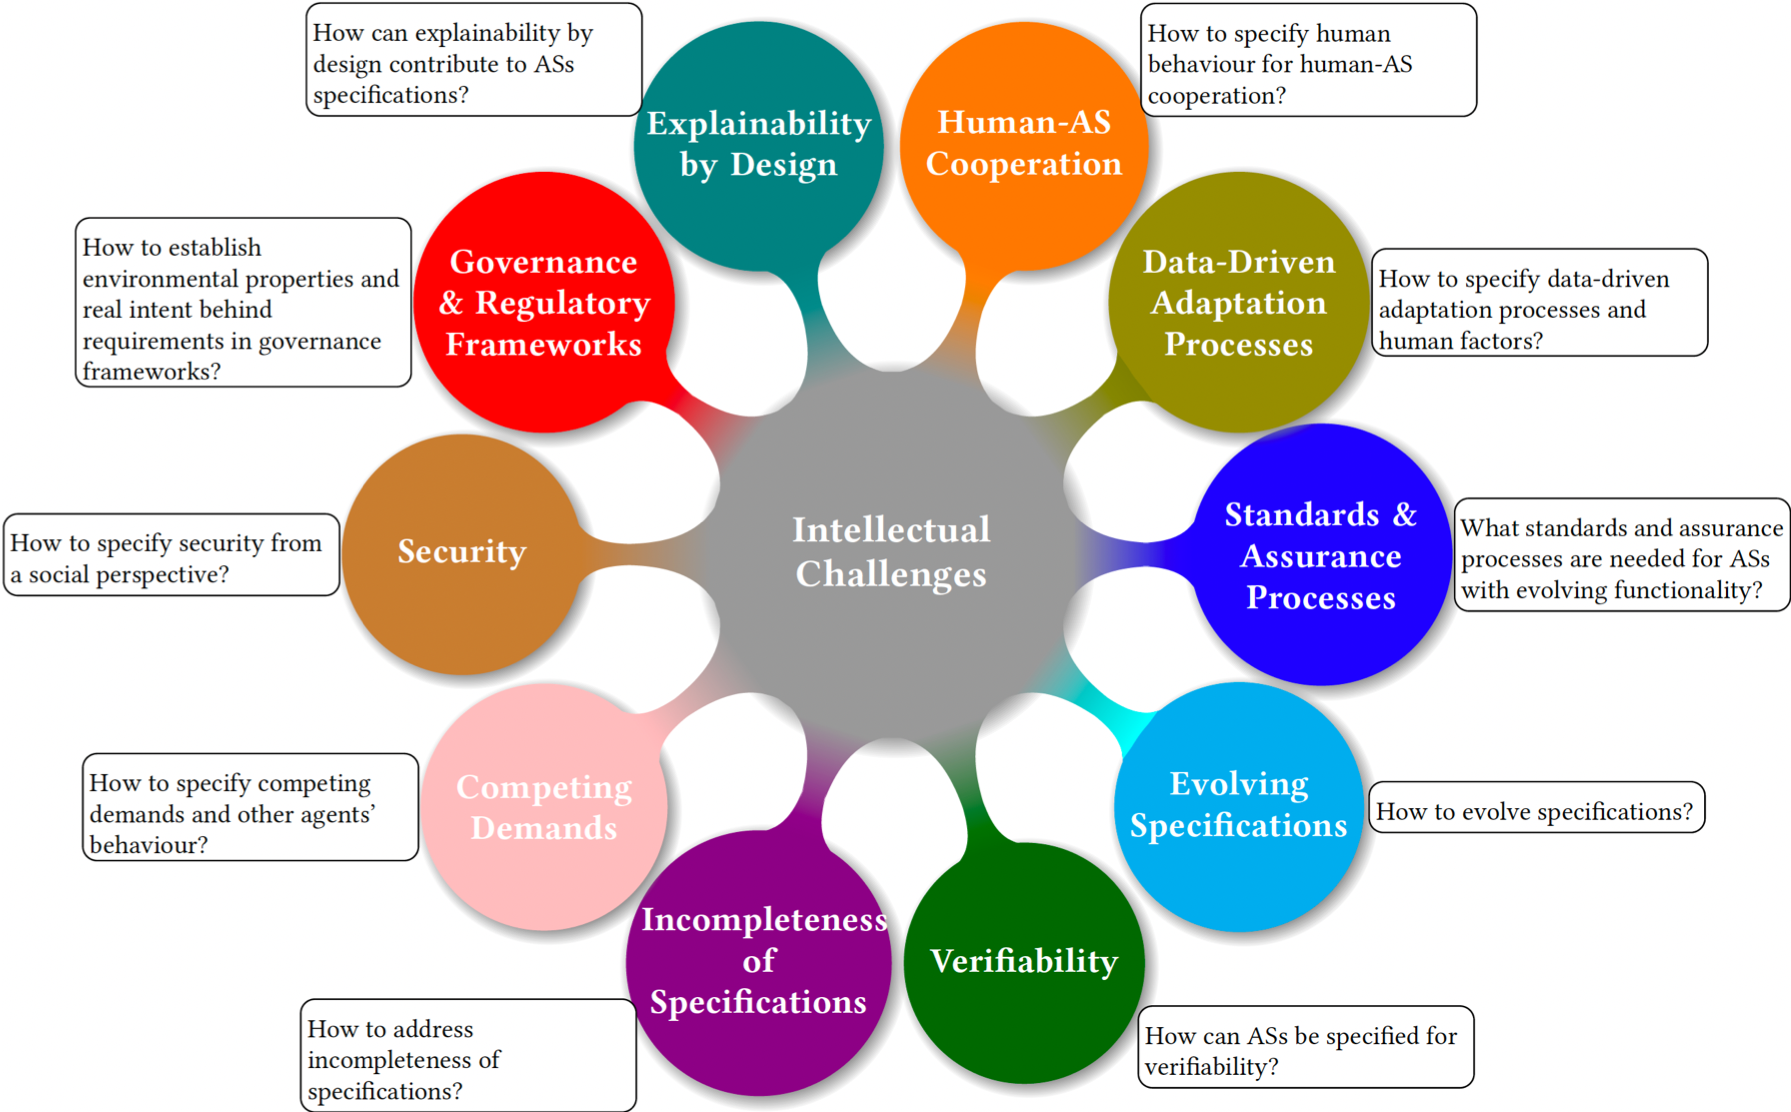
\includegraphics[width=0.85\textwidth]{figures/Intellectual-Challenges.png}%[width=0.95\textwidth]{figures/Intellectual-Challenges.png}
		\caption{Intellectual challenges for the AS community.}
		\label{Intellectual-challenges}
	\end{figure*}		
	
	%%------------------------------------------------------------------------------------------------------------------------------------------------------------------------------------------------------------------------------
	\begin{itemize}[leftmargin=0.5cm]
		\item \textbf{How to specify human behaviour for human-AS cooperation?}
	\end{itemize}
	How to model human behaviour to enable cooperation with AS is challenging but crucial for the resilience of the system as a whole. It is the diversity in human enactment that drives the uncertainty about what people do and don't do, and, subsequently, the way human behaviour can be specified. Knowing the mental state of others enables AS to steer a cooperation that is consistent with the needs of the AS, as well as to respond to the needs of human agents in an appropriate manner. 
	
	Different theories of human behaviours explain diversity in human action in different ways and by detecting various determinants of human behaviour. For example, a behaviourist approach suggests that every behaviour is a response to a certain stimulus~\cite{heimlich2008understanding}. Albeit true, this approach is restrictive in addressing the complexity of human behaviour, as well as the different ways that human behaviour develops during cooperation. To grasp that humans are embodied with purposes and goals that affect each other, the concept of joint-action can be introduced as ``a social interaction whereby two or more individuals coordinate their actions in space and time to bring about change in the environment''~\cite{sebanz2006joint}. Adapting it to human-robot interaction, this approach is suggestive of an interplay between humans and AS, such that what matters is not only how the AS understands the system but also how humans understand the way the autonomous agent behaves and is willing to cooperate~\cite{grigore:2013}. Thus, cooperation arises from a shared understanding between agents, which is a challenge to specify. 
	
	The social identity approach~\cite{spears2021social} induces this concept of a shared understanding by providing an explanation of human behaviour focusing on how social structures act upon cognition. It proposes that, alongside our personal identity, our personality - who we are, we also have multiple social identities based on social categories and groups. 
	Previous research has shown that social identities influence people's relation with technology~\cite{lee2001effect}. Sharing a social identity initiates pro-social behaviours, such as helping behaviours in emergency situations~\cite{drury2018role}. People adapt their behaviour in line with their shared identities, which in turn, enhances resilience. Specifying social identities to enable cooperation is challenging. It requires answering questions such as: how do we represent different identities and how do we reason about them? Following the social identity approach to specify identities for human-autonomous agent cooperation requires an investigation of how to operationalise social identity, a psychological state, into software embedded within AS.
	
	%Original contribution by the author/s:
	%
	%How to model human behaviour to enable cooperation with an autonomous systems is challenging but crucial for the resilience of the system as a whole. It is the diversity in human enactment that drives the uncertainty about what people do and don’t do, and, subsequently, the way human behaviour can be specified. Knowing the mental state of others enables autonomous systems to steer a cooperation that is consistent with the needs of the autonomous systems, as well as to respond to the needs of human agents in an appropriate manner. This knowledge guides an optimal course of action in a given context and can be used to identify mutually beneficial solutions. 
	%Different theories of human behaviours explain diversity in human action in different ways and by detecting various determinants of human behaviour. For example, a behaviourist approach suggests that every behaviour is a response to a certain stimulus~\cite{heimlich2008understanding}. Albeit true, this approach is restrictive in addressing the complexity of human behaviour~\cite{taylor2021explanation}, as well as the different ways that human behaviour develops during cooperation. To grasp that humans are embodied with purposes and goals that affect each other, the concept of joint-action was introduced as ``a social interaction whereby two or more individuals coordinate their actions in space and time to bring about change in the environment''~\cite{sebanz2006joint}. Adapting it to human-robot interaction, this approach is suggestive of an interplay between humans and autonomous systems, such that what matters is not only how the autonomous system understands the system but also how humans understand the way the autonomous agent behaves and is willing to cooperate. Thus, cooperation does not result from a reaction to actions but from a shared understanding between agents. 
	%The social identity approach~\cite{spears2021social} induces this concept of a shared understanding by providing an explanation of human behaviour focusing on how social structures act upon cognition. It proposes that, alongside our personal identity, our personality-who we are, we also have multiple social identities based on social categories and groups. We act in line with our social identity when this social identity is salient at a particular time~\cite{tajfel1982social}. Previous research has shown that social identities influence people’s relation with technology~\cite{lee2001effect}. Sharing a social identity initiates pro-social behaviours, such as helping behaviours in emergency situations~\cite{drury2018role}. People adapt their behaviour in line with their shared identities, which in turn, enhances resilience. Specifying social identities to enable cooperation is challenging. It requires an answer to a series of yet to be answered questions. How do we represent different identities and how do we reason about them? Following the social identity approach to specify identities for human-autonomous agent cooperation requires an investigation of how to operationalise social identity, i.e.~a psychological state, into software embedded within autonomous systems.
	
	%%------------------------------------------------------------------------------------------------------------------------------------------------------------------------------------------------------------------------------
	\begin{itemize}[leftmargin=0.5cm]
		\item \textbf{How to specify data-driven adaptation processes and human factors?}
	\end{itemize}
	Specifying, designing, implementing, and deploying interactive robot systems that are trustworthy for use in scenarios where humans and robots collaborate in close proximity is challenging, given that safety and reliability in such scenarios are of particular importance. Example scenarios include assisting people with activities of daily living such as mobility~\cite{SohDemiris2015} and dressing~\cite{GaoEtAl2020}, rehabilitation robotics, adaptive assistance in intelligent vehicles, robot assistants in care homes and hospital environments, among others. The intellectual challenge the AS community faces is the specification, design and implementation of trustworthy perceptual, cognitive, and behaviour generation processes that explicitly incorporate parametrizable models of human skills, beliefs, and intentions~\cite{Demiris2007}. 
	%
	These models are necessary for interactive assistive systems since they need to decide not only how but also when to assist~\cite{GeorgiouDemiris}. Given the large variability of human behaviour, the parameters of these user models need to be acquired interactively, typically from sparse and potentially noisy sensor data, a particularly challenging inverse problem. An additional challenge is introduced in the case of long-term human-robot interaction, where the assistive system needs to learn and take into consideration human developmental aspects, typically manifested in computational learning terms as model drift. 
	%
	As an example, consider the case of an assistive mobility device for children with disabilities~\cite{SohDemiris2015}: as the child's perceptual, cognitive, emotional and motor skills develop over time, their requirements for the type, amount and frequency of the provided assistance will need to evolve. Similarly, when assisting an elderly person or someone recovering from surgery, the distributions of the human data that the robot sensors collect will vary not only according to the context but also over time. 
	Depending on the human participant, and their underlying time-varying physiological and behavioural particularities, model drift can be sudden, gradual, or recurring, posing significant challenges to the underlying modelling methods. Principled methods for incorporating long-term human factors into the specification, design and implementation of assistive systems, that adapt and personalise their behaviour for the benefit of their human collaborator, remain an open research challenge. 
	
	%Original contribution by the author/s:
	% Removed references:
	% Demiris2009	
	%Designing, implementing, and deploying interactive robot systems that are trustworthy for use in scenarios where humans and robots collaborate in close proximity is challenging, given that safety and reliability in such scenarios are of particular importance. Example scenarios include assisting people with activities of daily living such as mobility \cite{SohDemiris2015} and dressing\cite{GaoEtAl2020}, rehabilitation robotics, adaptive assistance in intelligent vehicles, robot assistants in care homes and hospital environments, among others. The intellectual challenge this research community faces is the design and implementation of trustworthy perceptual, cognitive, and behaviour generation processes that explicitly incorporate parametrizable models of human skills, beliefs, and intentions\cite{Demiris2007}. These models are necessary for interactive assistive systems since they need to decide not only how but also when to assist\cite{Demiris2009, GeorgiouDemiris}.  Given the large variability of human behaviour, the parameters of these user models need to be acquired interactively, typically from sparse and potentially noisy sensor data, a particularly challenging inverse problem. An additional challenge is introduced in the case of long-term human-robot interaction, where the assistive system needs to learn and take into consideration human developmental aspects, typically manifested in computational learning terms as model drift. As an example, consider the case of an assistive mobility device for children with disabilities \cite{SohDemiris2015}: as the child’s perceptual, cognitive, emotional and motor skills develop over time, their requirements for the type, amount and frequency of the provided assistance will need to evolve. Similarly, when assisting an elderly person or someone recovering from surgery, the distributions of the human data that the robot sensors collect will vary not only according to the context but also over time, for example when assisting children to learn about and manage chronic conditions such as diabetes \cite{KapteinEtAl2022}.  Depending on the human participant, and their underlying time-varying physiological and behavioural particularities,  model drift can be sudden, gradual, or recurring, posing significant challenges to the underlying modelling methods. Principled methods for incorporating long-term human factors into the design and implementation of assistive systems, that adapt and personalise their behaviour for the benefit of their human collaborator, remain an open research challenge. 
	%-------------------------------------------------------------------------------------------------------------------------------------------------------------------------------------------------------------------
	
	\begin{itemize}[leftmargin=0.5cm]
		\item \textbf{What standards and assurance processes are needed for AS with evolving functionality?}
	\end{itemize}
	AS with \emph{evolving functionality}---the ability to adapt and change in function over time---pose significant challenges to current processes for specifying functionality. 
	Most conventional processes for defining system requirements assume that these are fixed and can be defined in a complete and precise manner before the system goes into operation. 
	Existing standards and regulations do not accommodate the adaptive nature of AS with evolving functionality. This is a key limitation~\cite{Fisher2020} that prevents promising applications such as swarm robots which adapt through emergent behaviour and UAVs with machine learning based flight control systems from deployment.
	
	For the use of swarm robots for item storage and distribution, ISO standards have been developed for the service robotics sector (non-industrial) (e.g.\ ISO 13482, ISO 23482-1, ISO 23482-2), and the industrial robotics sector (e.g.\ ISO 10218-1, ISO 10218-2, ISO/TS 15066). Although these industry standards focus on ensuring safety of robots at the individual robot level, they do not ensure safety or any other extra-functional property at the \emph{swarm} level that may arise through emergent behaviour.
	
	For airborne systems and in particular for UAVs, several industry standards and regulations have been introduced to specify requirements for system design and safe operation (e.g.\ DO-178C, DO-254, ED279, ARP4761, NATO STANAG 4671, CAP 722). However, none of these standards or regulations cover the types of machine learning based systems which are currently being developed to enable UAVs to operate autonomously in uncertain environments.
	
	The ability to adapt and to learn from experience are important abilities to enable AS to operate in real world environments. When one considers the existing industry standards, they are either implicitly or explicitly based on the V\&V model, which moves from requirements through design onto implementation and testing before deployment~\cite{Jia2021}. 
	However, this model is unlikely to be suitable for systems with the ability to adapt their functionality in operation; e.g.\ through interaction with other agents and the environment, as is the case with swarms; or through experience-driven adaptation as is the case with machine learning. AS with evolving functionality follow a different, much more iterative life-cycle. 
	Thus, there is a need for new standards and assurance processes that extend beyond design time and allow continuous certification at runtime~\cite{rushby:2008}.
	%
	% Original contribution by the author/s:
	%
	%Autonomous systems with \emph{evolving functionality}---the ability to change in function over time---pose significant challenges to current processes for specifying functionality. 
	%Most conventional processes for defining system requirements and characteristics assume that these are fixed and can be defined in a complete and precise manner before the system goes into operation. 
	%Existing standards and regulations do not satisfactorily address issues raised by them, which is a key limitation \cite{Fisher2020}. We discuss this using two application areas -- swarm robotics and UAVs.
	%
	%In the robotics domain, several safety standards have been developed by a technical committee of the ISO for the non-industrial (service) robotics sector (e.g. ISO 13482 \cite{ISO13482}, ISO 23482-1, ISO 23482-2 and for the industrial robotics sector (e.g. ISO 10218-1, ISO 10218-2, ISO/TS 15066). 
	%Different legal and regulatory requirements apply to different robot categories. 
	%In service robotics, ISO 13482 covers the hazards presented by the robots and devices for applications in non-industrial environments for providing services. 
	%ISO 23482-1 and ISO 23482-2 standards extend ISO 13482 with guidance and methods that can be used to test personal care robots.
	%On the other hand, in the industrial sector, ISO 10218-1 and ISO 10218-2 standards provide safety requirements for industrial robots and their integration.
	%Meanwhile, ISO/TS 15066 provides safety requirements for collaborative industrial robot systems
	%and work environment. 
	%Although these industry standards focus on ensuring safety of robots at the individual robot level, there are no standards to ensure safety or any other extra-functional property for \emph{swarms}.
	%
	%Meanwhile, for the airborne systems and in particular for UAVs, several industry standards and regulations have been introduced to ensure their safe operation. 
	%DO-178C \cite{DO-178C} is the primary standard for commercial avionics software development, which provides software considerations for the production of airborne systems and equipment. On the other hand, DO-254 provides guidance for the development of airborne electronic hardware. ED279 standard provides a framework to support designers when performing a functional hazard assessment process for an unmanned aircraft system. 
	%ARP4761 provides guidelines and methods for conducting the safety assessment process on civil airborne systems and equipment. 
	%NATO STANAG 4671 is intended to allow military UAVs to operate in other NATO members airspace. 
	%As for regulations within the UK, CAP 722 is the primary guidance document for the operation of unmanned aircraft systems. 
	%However, none of these standards or regulations provide safety considerations for machine learning components that enable evolving functionality.
	%
	%Furthermore, when one considers the existing industry standards, they are either implicitly or explicitly based on the V-model, which moves from requirements through design onto implementation and testing \cite{Jia2021}. 
	%For systems with the ability to adapt their functionality, this approach alone is unlikely to be suitable. 
	%For instance, the development of machine learning-based components of a UAV follows a different, much more iterative life-cycle. Therefore, there is a need for new standards and guidance that better reflect the life-cycle of autonomous systems with evolving functionality \cite{Hawkins2021}.
	
	%%------------------------------------------------------------------------------------------------------------------------------------------------------------------------------------------------------------------------------
	\begin{itemize}[leftmargin=0.5cm]
		\item \textbf{How to evolve specifications?}
	\end{itemize}
	Every typical AS undergoes changes over its lifetime that require going beyond an initially specified spectrum of operation --- despite the observation that this spectrum is typically quite large for AS in the first place~\cite{wilson2019amalgamation}. The evolution of trustworthy AS may concern changes of the requirements of their functional or non-functional properties, changes of the environment that the AS operate in, and changes in the trust of users and third parties towards the AS. 
 
    Initial specifications of the AS may no longer reflect the desired properties of the system or they may fail to accurately represent its environment. The evolution of specifications presents challenges in balancing the autonomy of the system.
	
    % JOR: I am commenting out the following paragraph as I don't see the evolution of specifications here, 
    % it seems to deal with the evolution of AS behavior (which is topic of the previous section).
    
    %Pursuing particular methods of evolution can make the task of specification easier. Some approaches (e.g. \cite{francesca2014automode}) allow systems to evolve behaviours from sets of predefined modules. These sub-modules can be independently specified and once the behaviour is evolved these independent specifications could be aggregated to form a valid overarching specification for the system. Similarly, adaptation can be limited to a few specified behaviour states or traits which are modified reactively \cite{wilson2019amalgamation}. If configured effectively, such systems should remain within the envelope of initial specification as the system evolves or adapts within its given constraints. Designing evolvable systems in this way will not only make specifying a system an easier task but will also make the system more transparent, understandable, and potentially more trustworthy.

    % new part on trustworthy AS emphasis
    While any non-trivial system requires evolution and maintenance~\cite{Mens08}, some challenges are exacerbated for trustworthy AS. As an example, observed changes in trust towards the AS might require changes to behaviour specifications, even if the AS operations are perfectly safe. Conversely, required changes to specifications might have negative impacts on future trust towards the AS. New methods will be required to efficiently deal with the various dimensions of trust in evolution of specifications.

    One dimension of trust relates to transparency towards developers of AS specifications. Approaches that compare evolving specifications on a syntactical level, as currently done for code, or on based on metrics, as currently done for AI models, are likely no longer sufficient for effective maintenance. Analysis will need to scale beyond syntactic differences to include also semantic differences~\cite{MaozR18} and allow for efficient analysis of the impact of changes on the level of systems rather than artefacts. New techniques to compare specifications of AS are required that identify, present, and explain differences as well as their potential impact on the system's trustworthiness.
	
	%Original contribution by the author/s:
	%Every non-trivial system undergoes changes over its lifetime. The evolution of trusted autonomous systems may concern changes of the requirements of their functional or non-functional properties, changes of the environment that it operates in, and changes in the trust of users towards the system. Initial specifications of the system may no longer reflect the desired properties of the system and fail to represent its actual environment.
	%
	%Self-adaptive systems~\cite{SalehieT09} constitute a special case of evolving systems where adaptation of the system is initiated from within itself. These systems require a tight coupling between the specification and implementation.
	%
	%Pursuing particular methods of evolution can make the task of specification easier. Some approaches, such as \cite{francesca2014automode}, allow systems to evolve behaviours from sets of predefined modules. These sub-modules can be independently specified and once the behaviour is evolved these independent specifications could be aggregated to form a valid overarching specification for the system. Similarly, adaptation can be limited to a number of specified behaviour states or traits which are modified reactively \cite{wilson2019amalgamation}. If configured effectively, such systems should remain within the envelope of initial specification as the system evolves or adapts within its given constraints. Designing evolvable systems in this way will not only make specifying a system an easier task but will also make the system more transparent, understandable and potentially more trustworthy.
	%
	%While a lot of work has been done to analyse, repair, explain, or simulate specifications little work has been to compare specifications, detect differences, and analyse their impact on the specified system. The comparison of complex specifications where small syntactic changes may have a large impact on their semantics calls for a semantic rather than syntactic comparison~\cite{MaozRR14j}. These semantic comparisons, e.g., as explored for Alloy~\cite{RingertW20}, may determine semantic equality despite syntactic changes, refinement of specifications, and concrete witnesses of changes.
	%
	%To summarize, one challenge in evolving specifications is to discover and faithfully represent changes to the system or its environment in specifications. 
	%%Approaches include \cite{0041035} 
	%Another challenge is the analysis of changes to specifications to explore and understand the impact of changes to specifications.
	%%------------------------------------------------------------------------------------------------------------------------------------------------------------------------------------------------------------------------------
	%%------------------------------------------------------------------------------------------------------------------------------------------------------------------------------------------------------------------------------
	\begin{itemize}[leftmargin=0.5cm]
		\item \textbf{How can AS be specified for verifiability?}
	\end{itemize}
	%	
	% Version edited by Kerstin 
	For a system to be {\em verifiable\/}, a person or a tool needs to be able to check its correctness~\cite{ISO24765:2017} with respect to its requirements and specification. 
	% Potentially we may need to say what we mean by correctness - the standard includes "correctness" too. 
	The main challenge is in specifying and designing the system in such a way that this process is made as easy and intuitive as possible.
	%
	For AS in particular, specific challenges include 
	%
	(i) capturing and formalising requirements including functionality, safety, security, performance and, beyond these, any additional non-functional requirements purely needed to demonstrate trustworthiness; 
	%	 
	(ii) handling flexibility, adaptation and learning; and 
	%
	% KIE: factored into the text below.
	%	In order to provide holistic verification results for an AS, different aspects of the system design need to be modelled and their interactions need to be analysed. These aspects are heterogeneous in nature and involve diverse domain abstractions. Hence, an autonomous system's specification should accommodate this heterogeneity and support the diverse domain abstraction. Ideally, such abstractions should be captured in notations that are most natural to domain experts.
	%
	(iii) managing the inherent complexity and heterogeneity of both the AS and the environment it operates in. 
	
	Specifications need to represent the different aspects of the overall system in a way that is natural to domain experts, facilitates modelling and analysis, provides transparency of how the AS works and gives insights into the reasons that motivate its decisions. 
	%
	To specify for verifiability, a specification framework will need to offer a variety of domain abstractions to represent the diverse, flexible and possibly evolving requirements AS are expected to satisfy. 
	%
	Furthermore, the underlying verification framework should connect all these domain abstractions to allow an analysis of their interaction. This is a key challenge in specification for verifiability in AS.
	
	AS can be distinguished using two criteria: the degree of autonomy and adaption, and the criticality of the application which can range from harmless to safety-critical. 
	We can consider which techniques or their combinations are needed for V\&V at the different stages of the system life-cycle. 
	When AS operate in uncontrolled environments, where there is a need for autonomy, learning and adaptation, the need for runtime V\&V emerges. 
	There, a significant challenge is finding rigorous techniques for the specification and V\&V of safety-critical AS where requirements are often vague, flexible and may contain uncertainty and fuzziness. 
	V\&V at design time can only provide a partial solution, and more research is needed to understand how best to specify and verify learning and adaptive systems by combining design time with runtime techniques. 
	Finally, identifying the design principles that enable V\&V of AS is a key pre-requisite to promote verifiability to a first-class design goal alongside functionality, safety, security, and performance.
	
	% Jan Ringert and Mohammad Mousavi's edited version of Dhaminda's and Kerstin's version:
	%In order to provide holistic and verification results for an autonomous system, different aspects of the system design need to be modelled and their interactions need to be analysed. These aspects are heterogeneous in nature and involve diverse domain abstractions. Hence, an autonomous system’s specification should accommodate this heterogeneity and support the diverse domain abstraction. Ideally, such abstractions should be captured in notations that are most natural to domain experts. In addition to providing a rich and diverse specification framework, the underlying verification framework should connect these diverse domain abstractions and should be able to analyse their interaction. This is a key challenge in specification for verifiability in autonomous systems.   
	%Moreover, there some additional challenges to be overcome in autonomous system’s specification for verifiability: (i) capturing and formalising requirements including functionality, safety, security, performance and, beyond these, any additional requirements purely needed to demonstrate trustworthiness;  (ii) capturing these requirements in the presence of flexibility, adaptation and learning: as ASs are equipped with mechanisms to evolve their functionality in response to internal and external changes, any adaptations during operation may change or entirely invalidate evidence obtained previously to demonstrate trustworthiness and (iii) managing the complexity of both the AS and the environment it operates in. To enhance verifiability we need methods to safely abstract complexity which will facilitate V&V, enable transparency of how ASs work, and give insights into the reasons that motivate their decisions.  
	%
	%ASs can be distinguished using two criteria: the degree of autonomy and adaption, and the criticality of the application which can range from harmless to safety-critical. We can consider which techniques or their combinations are needed for V&V at the different stages of the system life-cycle. When ASs operate in uncontrolled environments, where there is a need for autonomy, learning and adaptation, the need for runtime V&V emerges.  There, a significant challenge is finding rigorous techniques for the specification and V&V of safety-critical ASs where requirements are often vague, flexible and may contain uncertainty and fuzziness. V&V at design time can only provide a partial solution, and more research is needed to understand how best to verify learning and adaptive ASs including both at design time and at runtime techniques. 
	%
	%To address the verifiability research challenges, a combination of existing specification and modelling approaches is needed to capture the diverse, flexible and evolving requirements of ASs. Thus, a framework for V&V should integrate verifiability concerns to support  the software development process and serve as reference for V&V. Finally, capturing the design principles that enable V&V of AS is a key pre-requisite to promote verifiability to a first-class design goal alongside functionality, safety, security and performance. 
	%	
	%-------------------------------------------------------
	% Jan Ringer's original contribution
	%The vision of the verifiability node is to enable domain experts to use the most suitable abstractions, specifications, and tools for the verification task at hand. 
	%Many aspects of autonomous systems, e.g., functionality, security, or reliability, require their own formalisms and abstractions. Existing tools work with particular abstraction to provide verification results. 
	%However, we must be able to verify different aspect of these systems and how they operate together to enable trust:
	%Our goal is to develop a \textbf{unifying framework that will integrate and coalesce rigorous verification techniques of autonomous systems to quickly and easily verify complex autonomous systems}. 
	%We will achieve this outcome through a multi-disciplinary technical \textbf{research  programme} that seeks to: 
	%
	%\begin{enumerate}
	%	\item[\textbf{(a)}] \textbf{Classify} and relate verifiability concepts, notations, and techniques for autonomous systems.
	%	\item[\textbf{(b)}] \textbf{Design} the algorithms and techniques to integrate verification across disciplinary domains.
	%	\item[\textbf{(c)}]  \textbf{Create} an ecosystem of verification techniques concerning aspects such as functionality, resilience, security, and ethics. 
	%\end{enumerate} 
	%
	%To achieve this flexibility the verifiability node is developing a unifying framework for specification languages, their semantics, compositions, and transformations. 
	
	%%------------------------------------------------------------------------------------------------------------------------------------------------------------------------------------------------------------------------------
\begin{itemize}[leftmargin=0.5cm]
		\item \textbf{How to address incompleteness of specifications of AS?}
	\end{itemize}
	Incompleteness is a common property of specifications. Only the use of suitable abstractions allows for coping with the complexity of systems~\citep{Kramer07}. However, there is an important difference in the incompleteness introduced by abstractions, the process of eliminating unnecessary detail to focus e.g.\ on behavioural, structural, or security-related aspects of a system, and the incompleteness related to the purpose of the specification, i.e.\ the faithful representation of the system in an abstraction.
	
	On the one hand, if the purpose of creating and analysing a specification is to examine an AS and to learn about possible constraints, then incompleteness of the AS representation in the specification is important as it allows for obtaining feedback with low investment in specification development~\cite{Jackson19}, e.g. for the reduction of ambiguities. 
	%
	On the other hand, if the purpose of the specification is to prove a property, then incompleteness of the AS representation may lead to incorrect analyses results manifesting in false positives or false negatives. False positives are often treated by adding the missing knowledge to the specification of AS. For example, verifying the specification of an infusion pump reported a false positive due to (incompleteness)~\cite{HarrisonMCC17}. The specification had to be changed to a ``much more complex''~\cite{HarrisonMCC17} one to remove the false positive.

    One way of addressing incompleteness are partial models~\cite{CiolekBDPU17,WeiGC11,FamelisSC12} where models and analyses are extended with modalities qualifying their completeness. The various approaches provide analysis of either syntactic properties~\cite{FamelisSC12} or behavior refinements~\cite{WeiGC11}. Combinations and extensions to rich specification languages for AS are part of this research challenge.
	
	In the context of synthesis rather than verification the incompleteness of AS specifications can manifest itself in the construction of biased or incorrect systems. 
    %Potentially, synthesis may simply fail if necessary assumptions on the environment are missing. 
	%
	As an example, consider the specification of a robot operating in a warehouse~\cite{MaozR18robot}. The specification requires that the robot never hit a wall. With no assumptions about the environment, the synthesizer would take the worst-case view, i.e.\ walls move and hit the robot, and consequently report that no implementation exists. Adding the assumption that walls cannot changes the outcome of the synthesis. 
	%Similarly, without this assumption, a false positive result can also be expected during verification. 
	Interestingly, when formulating requirements for humans, common sense allows us to cope with this type of incompleteness. 
	%
	However, the automated analysis of specifications for AS brings with it the challenge of identifying and handling (all) areas of incompleteness.
	
	%----------------------------------------------------------------------------------------------------------------
	%Reviewed Version - 2022/06/22:
	%	Incompleteness is a common property of specifications. Only the use of suitable abstractions allows for coping with the complexity of systems~\citep{Kramer07}. However, there is an important difference in the incompleteness introduced by abstractions, the process of eliminating unnecessary detail to focus e.g.\ on behavioural, structural, or security-related aspects of a system, and the incompleteness related to the purpose of the specification, i.e.\ the faithful representation of the system in an abstraction.
	%	
	%	On the one hand, if the purpose of creating and analysing a specification is to examine a system and to learn about possible constraints, then incompleteness (``partiality'' in~\cite{Jackson19}) of the representation in the specification is important as it allows for obtaining feedback with low investment in specification development, e.g. for the reduction of ambiguity~\cite{Jackson19}. 
	%	%
	%	On the other hand, if the purpose of the specification is to prove a property, then incompleteness of the representation may lead to incorrect analyses results. These incorrect analysis results may manifest in false positives or false negatives. False positives are often treated by adding the missing knowledge to the specification. For example, consider the specification of an infusion pump from~\cite{HarrisonMCC17} and the property that all actions are reversible. The specification reported a false positive due to an advanced handling of overflows that was missing from the specification (incompleteness). The property in the specification had to be changed to a ``much more complex'' one~\cite{HarrisonMCC17} to remove the false positive.
	%
	%	In addition to analysis tasks, specifications are also used in synthesis tasks. This is where the incompleteness of the specifications can manifest itself in the construction of biased or incorrect systems. Potentially, the synthesis of ASs from incomplete specifications may simply fail if assumptions on the environment are incomplete. 
	%	%
	%	As an example, consider a robot operating in a warehouse~\cite{MaozR18}. The specification requires that the robot never hit a wall. With no assumptions about the environment, the synthesizer would take the worst-case view, i.e.\ walls move and hit the robot, and consequently report that the specification is not realisable and no implementation exists. Adding the assumption that walls cannot move as an environment constraint changes the outcome of the synthesis. 
	%	Similarly, without this assumption, a false positive result can also be expected during verification. 
	%	Interestingly, when formulating requirements for humans, common sense allows us to cope with this type of incompleteness. 
	%	%
	%	However, the automated analysis of specifications brings with it the challenge of identifying (all) areas of incompleteness.
	%----------------------------------------------------------------------------------------------------------------
	%Original contribution by the author/s:
	%Incompleteness is a necessary property of specifications. Only the use of suitable abstractions allows for coping with the complexity of systems~\citep{Kramer07}. However, there is an important difference in the incompleteness introduced by choosing abstractions, e.g., focusing on behavioral, structural, or security-related aspects of a system, and incompleteness with respect to the purpose of the specification, i.e., the faithful representation of the system given the chosen abstraction\footnote{The case where a chosen abstraction does not fit the purpose of the specification, e.g., the purpose is to rule out collisions of robots, but the abstraction ignores actuator inaccuracies, is out of the scope of this discussion.}. 
	%
	%On the one hand, if the purpose of creating and analysing a specification is to explore a system and to learn about possible constraints, e.g., as done with lightweight formal methods tools like Alloy~\cite{Jackson19}, then incompleteness of the representation in the specification is important as it allows for flexibility and quick gains. On the other hand, if the purpose of the specification is to prove a property and certify a system, then incompleteness of the representation may lead to incorrect analyses results. These incorrect analysis results may lead to false positives or false negatives. False positives can usually be fixed by adding the missing knowledge to the specification. As an example for a false positive consider the specification of an insulin pump from~\cite{HarrisonMCC17} and the property that all actions are reversible. The specification reported a false positive due to an advanced handling of overflows in the insulin pump and the specification had to be extended.
	%
	%In addition to analysis tasks, specifications are also used in synthesis tasks. In those cases the incompleteness of specifications may manifest in building biased or incorrect systems. Prominent examples include the bias of AI systems making autonomous decisions in health care~\cite{science.aax2342}. Other examples were observed in the area of program repair~\cite{GazzolaMM19} where initial work mainly relied on sets test cases (which in many cases represent incomplete specifications) producing incorrect repairs~\cite{QiLAR15,SmithBGB15}. 
	%
	%More general, the synthesis of autonomous systems from incomplete specifications may simply fail if assumptions on the environment are incomplete. As an example, consider a simple robot operating in a warehouse. The robot has sensors to detect obstacles and the specification requires the robot to never hit a wall. The synthesizer would report that the specification is not realizable and no implementation exists. The worst-case expectation of synthesis, if nothing else is specified, would be for walls to move and hit the robot. The environment needs to be further constrained by adding the natural assumption that walls cannot move\footnote{Additional challenges of writing specifications for reactive synthesis are described in~\cite{MaozR18}.}. In the case of verification, we can similarly expect a false positive result without this assumption. 
	%Interestingly, when formulating requirements to be read and understood by humans one would likely not formalize these assumptions necessary in specifications for autonomous systems. 
	%
	%To summarize, one challenge arising from automated analysis of specifications is to capture and encode implicit knowledge and common understanding available to humans into formal specifications. This includes to detect issues that were forgotten to specify and to disambiguate multiple plausible interpretations.
	
	
	%%------------------------------------------------------------------------------------------------------------------------------------------------------------------------------------------------------------------------------
	\begin{itemize}[leftmargin=0.5cm]
		\item \textbf{How to specify competing demands and other agents' behaviour?}
	\end{itemize}
	Conventional approaches to V\&V for AS may seek to attain coverage against a specification to demonstrate assurance of functionality and compliance with safety regulations or legal frameworks. 
	% Shane's comment: Is it technically correct to subsititue specifications for requirements in the previous sentence? This would help tie into the theme of the paper.
	Such properties may be derived from existing legal or regulatory frameworks, e.g.\ the UK Highway Code for driving, which can then be converted into formal expressions for automatic checking~\cite{harper2021safety}.
	
	But optimal safety does not imply optimal trust, and just because an AS follows rules does not mean that it will be accepted as a trustworthy system in human society. Other factors of trustworthiness should be considered, such as reliability, robustness, cooperation and performance. 
	%
	We can also say that strictly following safety rules may even be detrimental to other trustworthy properties, e.g.\ performance. 
	%
	Consider an automated vehicle trying to make progress through a busy market square full of people slowly walking across the road uncommitted to the usual observation of road conduct. 
	%
	The \emph{safest} option for the AS is to wait until the route ahead is completely clear before moving on, as by taking this option you do not endanger any other road user. However, \emph{better performance} may be to creep forward in a bid to promote your likelihood of success.
	%
	Driving then, is much more than following safety rules, which makes this a particularly hard specification challenge. In this scenario an assertive driving style would make more progress than a risk-averse one. 
	%
	
	
	In reality there will be significantly more considerations than just safety and performance, but this example illustrates the principle of conflicting demands between assessment standards. 
	%
	Consideration of other agents, such as properties of fairness or cooperation, would lead to a more trustworthy system. 
	%
	%In the language of game theory, assessing the payoff between a number of possible outcomes may indicate the fairest action to take. An assessment of the above \emph{busy market scenario} using game theory naturally lends itself to providing such an insight and may also give specification writers more freedom to express such complex properties. 
	Additionally, the interaction of AS with people may require insight into \emph{social norms} of which there is no written standard by which these can be judged. Will the task of specification first require a codex of social interaction norms to be drawn together to add to the standards by which trust can be measured? 
	%
	Specifications would need to be written with reference to these standards, regulations and ethical principles, some of which do not currently exist, in order to ensure that any assessment captures the full spectrum of these trustworthiness criteria. 
	%Trustworthiness could therefore be seen as a \emph{meta-property}, comprised of many criteria including safety but also reliability, security, usability, adoption and fairness amongst others~\cite{10.1145/3448248}. 
	%%
	%Earning trust will require satisfaction of these additional trustworthy criteria and along with it must come the standards by which they are judged. 
	%%
	%The existing standards for driving safety can be used to assess safe driving behaviour of an AS. Safe driving is therefore one aspect of trustworthiness that we can currently provide a testable assessment of, but is only a part of the entire trust meta-property. 
	%%
	%Specifying for trustworthiness will inevitably overlap with laws, societal norms, regulations, human factors, standards on personal data collection and use, cybersecurity and committees to ensure unbiased and ethical standards are upheld. 
	%%
	
	A further challenge to specification will not just be to capture the full gamut of properties for trustworthiness, but also in deciding a hierarchy through the meta-trustworthiness stack. 
	%
	Similar to the Asimov law of robotics, where safety to humans will outrank that of self-preservation of the robot, a similar system of hierarchy may be required.
	%
	It may also be useful to consider which aspects of the specification have soft or hard limits, i.e.\ which are inviolable and which may be traded-off against other properties as in the case of safety versus performance or other competing demands. 
	
	%Original contribution by the author/s:
	%
	%
	%-------------
	%Conventional approaches to verification and validation for autonomous systems may seek to attain coverage against a set of requirements to demonstrate assurance of functionality and compliance with safety regulations or legal frameworks. 
	%%
	%Such properties may be derived from existing legal or regulatory frameworks, e.g. the UK Highway Code~\cite{highwayCode} for driving, which can then be converted into logical computer expressions used as a tool for assessment using; geospatial database queries~\cite{harper2021safety}, higher order logic~\cite{rizaldi}, or linear temporal logic~\cite{esterle2020}.
	%
	%
	%But optimal safety does not imply optimal trust, and just because an autonomous system follows rules does not mean that it will be accepted as a trustworthy system in human society. 
	%%
	%We can also say that strictly following safety rules may even be detrimental to other properties, e.g. performance. 
	%%
	%Consider an autonomous vehicle trying to make progress through a busy market square full of people slowly walking across the road uncommitted to the usual observation of road conduct. 
	%%
	%The \emph{safest} option for the autonomous system is to wait until the route ahead is completely clear before moving on, as by taking this option you do not endanger any other road user. However, \emph{better performance} may be to creep forward in a bid to promote your likelihood of success.
	%%
	%Driving then, is much more than following safety rules and in this scenario an aggressive driving style would make more progress than a risk-adverse one. 
	%%
	%
	%
	%In reality there will be significantly more considerations than just safety and performance but this example illustrates the principle of conflicting demands between assessment standards. 
	%%
	%Consideration of other agents, such as properties of fairness or cooperation, would lead to a more trustworthy system. 
	%%
	%In the language of game theory, assessing the payoff between a number of possible outcomes may indicate the fairest action to take. An assessment of the above \emph{busy market scenario} using game theory naturally lends itself to providing such an insight and may also give specification writers more freedom to express such complex properties. 
	%
	%
	%Additionally, the interaction of autonomous systems with people may require insight into \emph{social norms} of which there is no written standard by which it can be judged. Will the task of specification first require a codex of social interaction norms to be drawn together to add to the standards by which trust can be measured? 
	%%
	%Specifications will need to be written with reference to these standards, regulations and ethical principles, some of which do not currently exist, in order to ensure that any assessment captures the full spectrum of these trustworthiness criteria.
	%
	%
	%Trustworthiness could therefore be seen as a \emph{meta-property}, comprised of many criteria including safety but also reliability, security, usability, adoption and fairness amongst others~\cite{10.1145/3448248}. 
	%%
	%Earning trust will require satisfaction of these additional trustworthy criteria and along with it must come the standards by which they are judged. 
	%%
	%The existing standards for driving safety can be used to assess safe driving behaviour of an autonomous system. Safe driving is therefore one aspect of trustworthiness that we can currently provide a testable assessment of, but is only a part of the entire trust meta-property. 
	%%
	%Specifying for trustworthiness will inevitably overlap with laws, societal norms, regulations, human factors, standards on personal data collection and use, cybersecurity and committees to ensure unbiased and ethical standards are upheld. 
	%%
	%
	%A further challenge to specification will not just be to capture the full gamut of trustworthiness properties, but also in deciding a hierarchy through the meta-trustworthiness stack. 
	%%
	%Similar to the Asimov law of robotics, where safety to humans will outrank that of self-preservation of the robot, a similar system of hierarchy is required.
	%%
	%It may also be useful to consider which aspects of the specification have soft or hard limits, i.e which are inviolable and which may be traded-off against other properties as in the case of safety versus performance or other competing demands. 
	%%
	%% This approach may allow conflicts between properties to be more easily resolved.	
	%%------------------------------------------------------------------------------------------------------------------------------------------------------------------------------------------------------------------------------
	\begin{itemize}[leftmargin=0.5cm]
		\item \noindent\textbf{How to specify security from a social perspective?} 
	\end{itemize}
	There are technical sides to security, but there are also social dimensions that matter when considering how an AS enforces its status as secure. In this context, security overlaps with trust. One can only be assured a system is secure, if one trusts that system. Public trust is a complex issue, shot through with media, emotions, politics, and competing interests. How do we go about specifying security in a social sense? 
	
	On the technical side, there are fairly specific definitions for specification which can be grasped and measured. From the social perspective, the possibility of specification relies on a network of shared assumptions and beliefs that are difficult to unify. In fact, much of the value from engagement over social specifications derives from the diversity and difference. 
	A predominant concern in social aspects of security is where data is shared between systems (social-material interactions).
	That is, whenever an AS communicates with a human being or an aspect of the environment. 
	Although these interactions have technical answers, to find answers that consider social science perspectives requires collaboration and agile methods to facilitate that collaboration.
	
	The human dimension means that it is not enough to specify technical components. Specifications must also capture believes, desires, fears and at times misinformation with respect to how those are understood, regarded and perceived by the public. For example, in what ways can we regard pedestrians as passive users of automated vehicles? How are automated vehicles regarded by the public, and how are pedestrians involved in automated mobility?
	
	The ethical challenges that emerge for AS security also relate to the legal and social ones. 
	The difficulty centres around how to create regulations and specifications on a technical level, that are also useful socially, facilitating responsiveness to new technologies that are neither simply techno-phobic nor passively accepting. 
	Doing so must involve both innovation and public input, so that the technology developed works for everyone. The ELSI (Ethical, Legal \& Social Implications) framework~\cite{Escalante2019} is an example of a framework aimed to engage designers, engineers, and public bodies in answering these questions. ELSI is an inherently cross-disciplinary set of approaches for tackling AS security, as many interrelated and entangled aspects. Specifying security requires connection, collaboration, and agile ethical methods.
	
	%Revised version by author on December 14, 2021:
	%There are technical sides to security, but there are also social dimensions that matter when thinking through how an AS solidifies its status as secure. In this context, security overlaps with trust. One can only be assured a system is secure if one trusts that system. Public trust is a complex issue, shot through with media, emotions, politics, and competing interests. How do we go about specifying security in a social sense? 
	%
	%On the technical side, there are fairly specific definitions for specification which can be grasped, and more, measured. From the social perspective, the possibility of specification relies on a network of shared assumptions and beliefs that are difficult to unify. In fact, much of the value from engagement over social specifications, derives from the diversity and difference. A predominant concern in social aspects of security is where data is shared between systems, what we call social-material interactions, that is, whenever an autonomous system communicates with a human being or an aspect of the environment. As already mentioned, these interactions have technical answers. To get at the answers that speak to social science perspectives requires collaboration, and agile methods to facilitate that collaboration.
	%
	%As soon as you introduce human-beings into the picture of Autonomous Systems, things get complicated, now you are not just dealing with instructions that you give to a device but dealing with believes, desires and fears sometimes misinformation, how those are understood, regarded and perceived by publics. For example, in what ways can we regard pedestrians as passive users of autonomous vehicles. How are autonomous vehicles regarded by publics, and how are pedestrians involved in automated mobility?
	%
	%What ethical challenges emerge for AS security also relate to the legal and social ones. The difficultly centers around how to create regulation and specification on a technical level, but also useful for social spaces, responsive to new technologies in a way that is neither simply techno-phobic nor passively accepting. Doing so must involve both innovation and public input. So, the technology that you receive is what works for everyone. To engage designers, engineers, and public bodies in answering these questions, we are using the ELSI framework. Standing for Ethical, Legal & Social Implications, this is an inherently cross-disciplinary set of approaches for tackling AS security as many interrelated and entangled aspects. Specifying security requires connection, collaboration, and agile ethical methods.
	
	
	%Original contribution by the author/s on October 27, 2021:
	%There are technical sides to security, but there are also social dimensions that matter when thinking through how an AS solidifies its status as secure. In this context, security overlaps with trust. One can only be assured a system is secure if one trusts that system. Public trust is a complex issue, shot through with media, emotions, politics, and competing interests. How do we go about specifying security in a social sense? 
	%
	%On the technical side, there are fairly specific definitions for specification which can be grasped, and more, measured. From the social perspective, the possibility of specification relies on a network of shared assumptions and beliefs that are difficult to unify. In fact, much of the value from engagement over social specifications, derives from the diversity and difference. A predominant concern in social aspects of security is where data is shared between systems, what we call social-material interactions... that is whenever an autonomous system communicates with a human being or an aspect of the environment. As already mentioned, these interactions have technical answers. To get at the answers that speak to social science perspectives, requires collaboration, and agile methods to facilitate that collaboration.
	%
	%As soon as you introduce human-beings as in the picture of Autonomous Systems, things get complicated, now you are not just dealing with instructions that you give to a device but dealing with believes, desires and fears sometimes misinformation, how those are understood, regarded and perceived by publics. For example, in what ways can we regard pedestrians as passive users of autonomous vehicles. How are autonomous vehicles regarded by publics, and how are pedestrians involved in automated mobility?
	%
	%What ethical challenges emerge for AS security also relate to the legal and social ones. The difficultly centers around how to create regulation and specification on a technical level, but also useful for social spaces, responsive to new technologies in a way that is neither simply techno-phobic nor passively accepting. Doing so must involve both innovation and public input. So, the technology that you receive is what works for everyone. To engage designers, engineers, and public bodies in answering these questions, we are using the ELSI framework. Standing for Ethical, Legal \& Social Implications, this is an inherently cross-disciplinary set of approaches for tackling AS security as many interrelated and entangled aspects. Specifying security requires connection, collaboration, and agile ethical methods.
	
	%%------------------------------------------------------------------------------------------------------------------------------------------------------------------------------------------------------------------------------
	\begin{itemize}[leftmargin=0.5cm]
		\item \textbf{How to establish environmental properties and real intent behind requirements in governance frameworks?}
	\end{itemize}
	Computer scientists treat specifications as precise objects, often derived from requirements by purging features such that they are defined with respect to environment properties that can be relied on regardless of the machine's behaviour. Emerging AS applications in human-centred environments can challenge this way of thinking, particularly so because the environment properties may not be fully understood, or because it is hard to establish if the real intent behind a requirement can be verified. These gaps should be addressed in governance frameworks in order to engender trust.
	
	For instance, in all of the domains mentioned above, we are increasingly seeing systems that are data-first and subject to continuous deployment. This has the interesting consequence that sometimes even the task requirements are really only given in terms of fit to observed human behaviour~\cite{topol2019high}, e.g.\ what does an expert say in radiology interpretation and does the AI-based AS match that~\cite{Freemann1872}. We see this as a crucial area for future development, as existing workflows depend on human interpretation of rules in crucial ways, whereas when AS perform the same decisions there is scope for significant disruption of these workflows due to potential gaps that become exposed.

	Furthermore, many emerging concerns such as fairness are not only difficult to formalise in the sense of software specification, but also their many definitions can be conflicting such that it is impossible to satisfy all of them in a given system~\cite{narayanan21fairness}. 
	
	AS of the future will need a combination of informal and formal mechanisms for governance. In domains such as automated vehicles, trustworthiness of the system may require a complete ecosystem approach~\cite{koopman2019certification} involving community-defined scenario libraries, enabling the greater use of simulation in verification, and independent audits via independent third parties. This calls for the development of new computational tools for performance and error characterisation, systematic adversarial testing with respect to a range of different specification types, and causal explanations that address not only a single instance of a decision but better expose informational dependencies that are useful for identifying edge cases and delineating operational design domains. 
	
	In addition to all of these technical tools, there is a need to understand the human-machine context in a more holistic manner, as this is really the target of effective governance. People's trust in an AS is not determined by technical reliability alone. Instead, the expectations of responsibility and accountability are associated with the human team involved in the design and deployment of the system, and the organisational design behind the system. A vast majority of system failures are really failures arising from mistakes made in this `outer loop'. Therefore, effective regulations must first begin with a comprehensive mapping of responsibilities that must be governed, so that computational solutions can be tailored to address these needs. Furthermore, there is a need for ethnographic understanding of AS being used in context, which could help focus technical effort on the real barriers to trustworthiness.
	
	%Original contribution by the author/s:
	%Computer scientists treat specifications as precise objects, often derived from requirements by purging features such that they are defined with respect to environment properties that can be relied on regardless of the machine's behaviour. Emerging autonomous systems applications  in human-centred environments can challenge this way of thinking, particularly so because the environment properties may not be fully understood, or because it is hard to establish if the real intent behind a requirement can be verified. These gaps should be addressed in governance frameworks in order to engender trust.
	%
	%For instance, in all of the domains mentioned above, we are increasingly seeing systems that are data-first and subject to continuous deployment. This has the interesting consequence that sometimes even the task requirements are really only given in terms of fit to observed human behaviour \cite{topol2019high}, e.g. what does an expert say in radiology interpretation and does the AI-based autonomous system match that \cite{Freemann1872}. Furthermore, many emerging concerns such as fairness are not only difficult to formalise in the sense of software specification, but also their many definitions can such that it is impossible to satisfy all of them in any system \cite{narayanan21fairness}. 
	%
	%It is clear that autonomous systems of the future will need a combination of informal and formal mechanisms for governance. In domains such as autonomous vehicles, trustworthiness of the system may require a complete ecosystem approach \cite{koopman2019certification} involving community-defined scenario libraries, enabling the greater use of simulation in verification, and independent audits via independent third parties. This calls for the development of new computational tools for performance and error characterisation, systematic adversarial testing with respect to a range of different specification types, and causal explanations that address not only a single instance of a decision but better expose informational dependencies that are useful for identifying edge cases and delineating operational design domains. 
	%
	%In addition to all of these technical tools, there is a need to understand the human-machine context in a more holistic manner, as this is really the target of effective governance. People's trust in an autonomous system is not determined by technical reliability alone. Instead, the expectations of responsibility and accountability are associated with the human team involved in the design and deployment of the system, and the organisational design behind the system. A vast majority of system failures are really failures arising from mistakes made in this `outer-loop'. Therefore, effective regulations must first begin with a comprehensive mapping of responsibilities that must be governed, so that computational solutions can be tailored to address some of these needs. Furthermore, there is a need for ethnographic understanding of autonomous systems being used in context, which could help focus technical effort on the real barriers to trustworthiness.
	%%------------------------------------------------------------------------------------------------------------------------------------------------------------------------------------------------------------------------------
	%\subsection{Explainability by design}
	
	%	\begin{itemize}[leftmargin=0.5cm]
		%		\item \textbf{Explainability by design}
		%	\end{itemize} 	
	\begin{itemize}[leftmargin=0.5cm]
		\item \textbf{How can explainability by design contribute to AS specifications?}
	\end{itemize} 	
	There are increasing calls for explainability in AS, with emerging frameworks and guidance~\cite{Hamon:2020} pointing to the need for AI to provide explanations about decision making. A challenge with specifying such explainability is that existing frameworks and guidance are not prescriptive: what is an actual explanation and how should an explanation be constructed? Furthermore, frameworks and guidance tend to be concerned with AI in general, and not AS.
	
%	A case study addressing regulatory requirements on explainability of automated decisions in the context of a loan application~\cite{Huynh:DGOV21} provided foundations for a systematic approach. Within this context, explanations can act as external detective controls, as they provide
%	specific information to justify the decision reached and help the user take corrective actions~\cite{Tsakalakis:CLSR21}. But explanations can also act as internal detective controls, i.e. a mechanism for organisations to demonstrate compliance to the regulatory frameworks they have to implement. 
%	Both~\cite{Huynh:DGOV21} and~\cite{Tsakalakis:CLSR21} provide systematic questions that an explanation designer needs to consider: What is the purpose of an explanation? What is the audience of an explanation? What is the information that it should contain? However, to adequately address these questions, explainability should not be seen as an after-thought, but as an integral part of the specification and design of a system, leading to explainability requirements to be given the same level of importance as all other aspects of a system. 
%	
%	The study and design of AS include many facets: not only black-box or grey-box AI systems, but also the various software and hardware components of the system, the curation and cleansing of datasets used for training and validation, the governance of such systems, their user interface and crucially the users of such systems with a view of ensuring that they do not harm but provide benefits to these users and society in general. There are typically a range of stakeholders involved, from the designers of the systems, to their hosts and/or owners, their users (consumers and operators), third-parties and increasingly regulators. In this context, many questions related to trustworthy AS (such as what is an actual explanation and how should an explanation be constructed? What is the purpose of an explanation? What is the audience of an explanation? What is the information that it should contain?) have to be addressed holistically, it no longer suffices to focus on the explainability of a black-box decision system, its behaviour needs to be explained, with more and less details, in the context of the overall AS.	

	A case study addressing regulatory requirements on explainability of automated decisions in the context of a loan application~\cite{Huynh:DGOV21} provided foundations for a systematic approach. Within this context, explanations can act as external detective controls, as they provide specific information to justify the decision reached and help the user take corrective actions~\cite{Tsakalakis:CLSR21}. But explanations can also act as internal detective controls, i.e. a mechanism for organisations to demonstrate compliance to the regulatory frameworks they have to implement. 
	%Both~\cite{Huynh:DGOV21} and~\cite{Tsakalakis:CLSR21} provide systematic questions that an explanation designer needs to consider: What is the purpose of an explanation? What is the audience of an explanation? What is the information that it should contain? 
	The study and design of AS include many facets: not only black-box or grey-box AI systems, but also the various software and hardware components of the system, the curation and cleansing of datasets used for training and validation, the governance of such systems, their user interface and crucially the users of such systems with a view of ensuring that they do not harm but provide benefits to these users and society in general. There are typically a range of stakeholders involved, from the designers of the systems, to their hosts and/or owners, their users (consumers and operators), third-parties and increasingly regulators. In this context, many questions related to trustworthy AS (such as what is an actual explanation and how should an explanation be constructed? What is the purpose of an explanation? What is the audience of an explanation? What is the information that it should contain? \cite{Huynh:DGOV21,Tsakalakis:CLSR21}) have to be addressed holistically, it no longer suffices to focus on the explainability of a black-box decision system, its behaviour needs to be explained, with more and less details, in the context of the overall AS. However, to adequately address these questions, explainability should not be seen as an after-thought, but as an integral part of the specification and design of a system, leading to explainability requirements to be given the same level of importance as all other aspects of a system. 
	
	In the context of trustworthy AS, emerging AS regulations could be used to drive the socio-technical analysis of explainability. A particular emphasis would have to be on the autonomy and the hand-over between systems and humans that characterise trustworthy AS. The audience of explanations will also be critical, from users and consumers to businesses, organisations and regulators. Finally, considerations for post-mortem explanations, in case of crash or disaster situations involving AS, should lead to adequate architectural design for explainability.
	
	%Original contribution by the author/s:
	
	%Increasingly, calls for explainability~\cite{Hamon:2020,gchq:2021}, as well as  emerging frameworks~\cite{Hamon:2020} and guidance ~\cite{ico:2020}  point to the need for Artificial Intelligence (AI) to provide explanations about the decisions it makes.  A challenge with existing frameworks and guidance is that they are not prescriptive: what is an actual explanation?   how   should an explanation be constructed? can it be constructed  computationally?  Furthermore,  frameworks and guidance tend to be concerned with AI in general, and not Autonomous Systems, which have a substantial overlap with AI but are distinct from AI.
	%
	%A case study addressing regulatory requirements on explainability of automated decisions in the context of a loan application~\cite{Huynh:DGOV21} provided foundations for a systematic approach. Within this context, explanations can act as external detective controls~\cite{Tsakalakis:CLSR21}, as they provide
	%specific information to justify the decision reached and help the user take corrective actions: ``The aim of these explanations is to provide data subjects with an adequate understanding about the decision so that they can exercise their corrective rights''~\cite{Tsakalakis:CLSR21}. But explanations can also act as internal detective controls~\cite{Tsakalakis:CLSR21}, i.e.,  a mechanism for organisations to demonstrate compliance to the regulatory frameworks they have to implement. 
	%Both~\cite{Huynh:DGOV21} and~\cite{Tsakalakis:CLSR21} provide   systematic questions that an explanation designer needs to consider: What is the purpose of an explanation? What is the audience of an explanation?  What is the information that it should contain? However, to adequately address these questions, explainability should not be seen as an after-thought, but as an integral part of the design of an application, leading to explainability requirements to be included in its design, like all its other aspects.  
	%
	%The PLEAD project (\href{https://plead-project.org/}{https://plead-project.org/}), ``Provenance-based and Legally-grounded Explanations for Automated Decisions'' project adopts a two-pronged approach to address this challenge. (1) Technologically, PLEAD decomposes the problem of explainability in two distinct parts,   logging “a record that describes the people, institutions, entities, and activities involved in producing, influencing, or delivering”~\cite{Moreau:prov-dm:20130430} an automated decision, and using that record to construct ``An explanation, as a targeted, personalised textual or visual artifact that provides a focused description of the behaviour of the system''.  A structure for this record already exists in the form of  PROV, a Recommmendation of the World Wide Web Consortium~\cite{Moreau:prov-dm:20130430}.  (2) Methodologically, PLEAD offers a socio-technical approach, involving autonomous systems stakeholders to understand various dimensions of an explanation (purpose, audience, trigger, minimum content, explanation examplar, ...), to which an ``explainability by design'' methodology is applied to construct the system able to generate explanations that can be evaluated by stakeholders, before  deployment and integration with the application.
	%
	%Explainability by design is a methodology that takes the stakeholder requirements for explainability as input, models application provenance, design queries, and constructs explanation plans, which can be all bundled up in a standalone component able to receive applications data and generate explanations addressing the requirements identified by the PLEAD socio-technical analysis.
	%
	%We have applied the methodology to systems providing explanations about decisions related to credit card applications and school allocations. These decisions are taken with various degrees of autonomy, in partnership with humans.  Preliminary evaluations are showing positive feedback from the participants.
	%
	%In the context of Trustworthy Autonomous Systems, emerging AS regulations could be used to drive the socio-technical analysis of explainability.  A particular emphasis would have to be on the autonomy and the hand-over between systems and humans that characterise  TAS systems.  The audience of explanations will also be critical, from users and consumers to businesses, organisations and regulators.  Finally, considerations for post-mortem explanations, in case of crash or disaster situation involving autonomous systems, should lead to adequate architectural design.
	
	
	%%------------------------------------------------------------------------------------------------------------------------------------------------------------------------------------------------------------------------------
	
	
	\section{Summary and Conclusions}\label{conclusions}	
	As AS are becoming part of our daily lives and interacting more closely with humans, we need to build systems worthy of trust regarding safety, security, and other non-functional properties. In this paper we have first examined AS domains of different levels of maturity and then identified their specification challenges and related research directions. 
	One of these challenges is the formalisation of knowledge easily grasped by humans so that it becomes interpretable by machines. Prominent examples include the specification of driving regulations for AVs, and the specification of human knowledge expertise in the context of AI-based medical diagnostics. 
	%
	How to specify and model human behaviour, intent and mental state is a further challenge that is common to all domains where humans interact closely with AS, such as in human-robot collaborative environments as found in smart manufacturing. 
	%
	%-------
	Alternative approaches involve the specification of norms to characterise the desired behaviour of AS, which regulate what the system should do or should not do. An emerging direction of research is the design of monitors to observe the system and check compliance with norms~\cite{Criado:2018}. 
	%-----
	%
	The example of swarm robotics raises the need and challenge to specify behaviour that emerges at the system level and relies on certain actions of the entities that form the system with each other and their environment. 
	
	Beyond the technical aspects, across the specific AS domains, are research challenges related to governance and regulation for trustworthiness, requiring a holistic and human centred approach to specification focused on responsibility and accountability, and enabling explainability from the outset. 
	%
	Fundamental to specifying for trustworthiness is a sound understanding of human behaviour and expectations, as well as the social and ethical norms applicable when humans directly interact with AS. 
	% 
	As for future work, an interesting extension of this paper would be to produce a classification of properties to be specified for trustworthiness under the different intellectual challenges discussed (e.g. socio-technical properties of explainability are purpose, audience, content, timing and delivery mechanism of explanations). 
	
	We conclude that specifying for trustworthiness requires advances on the technical and engineering side, informed by new insights from social sciences and humanities research. Thus, tackling this specification challenge necessitates tight collaboration of engineers, roboticists and computer scientists with experts from psychology, sociology, law, politics and economics, as well as ethics and philosophy. Most importantly, continuous engagement with regulators and the general public will be key to trustworthy AS.
	
	\begin{acks}
%		This article is a result of the fruitful discussions held at the Specifying for Trustworthiness workshop during the Trustworthy Autonomous Systems (TAS) All Hands Meeting in September 2021. 
		The work presented in this paper has been supported by the UK Engineering and Physical Sciences Research Council (EPSRC) under the grants: [EP/V026518/1], [EP/V026607/1], [EP/V026747/1], [EP/V026763/1], [EP/V026682/1], [EP/V026801/2] and [EP/S027238/1]. Y.D. is also supported by a RAEng Chair in Emerging Technologies [CiET1718\textbackslash46].
	\end{acks}
	
	\bibliographystyle{ACM-Reference-Format}
	\bibliography{TAS-Spec-Bibliography}
	
\end{document}
\endinput
